\section*{Общая характеристика работы}

\newcommand{\actuality}{{\textbf{\actualityTXT}}}
\newcommand{\progress}{{\textbf{\progressTXT}}}
\newcommand{\aim}{{{\textbf\aimTXT}}}
\newcommand{\tasks}{{\textbf{\tasksTXT}}}
\newcommand{\novelty}{{\textbf{\noveltyTXT}}}
\newcommand{\influence}{{\textbf{\influenceTXT}}}
\newcommand{\methods}{{\textbf{\methodsTXT}}}
\newcommand{\defpositions}{{\textbf{\defpositionsTXT}}}
\newcommand{\reliability}{{\textbf{\reliabilityTXT}}}
\newcommand{\probation}{{\textbf{\probationTXT}}}
\newcommand{\contribution}{{\textbf{\contributionTXT}}}
\newcommand{\publications}{{\textbf{\publicationsTXT}}}



{\actuality} 
\todo{В настоящее время существенный интерес проявляется к разработке автономных робототехнических систем, предназначенных для передвижения в жидкости. Как правило, такие устройства перемещаются с использованием гребных винтов или подвижных лопастей. Но встречаются и другие устройства, реализующие «нетрадиционные» способы передвижения. Один из таких типов устройств – это локомоционный робот с внутренним механизмом, у которого в процессе движения внешняя оболочка остается неизменной, и отсутствуют приводные элементы, взаимодействующие непосредственно с жидкостью или воздухом над ее поверхностью. При этом движение осуществляется за счет работы внутреннего механизма, изменяющего положение центра масс системы и (или) гиростатический момент.
Данный тип роботов обладает рядом преимуществ по сравнению с другими «традиционными» конструкциями: изолированность рабочих узлов от жидкости, возможность полной гидроизоляции, низкий уровень гидродинамического шума при передвижении, повышенная маневренность. Эти особенности локомоционных роботов с внутренним механизмом позволяют применять их для исследования и мониторинга в жидкости с высокими экологическими нормами, в легковоспламеняющихся средах, в условиях высокого гидростатического давления.
Данный способ передвижения в жидкости является новым, как с точки зрения гидродинамики, так и мобильной робототехники, что подтверждается наличием небольшого количества теоретических работ в данном направлении. Теоретические исследования движения таких систем (с переменным распределением массы) в идеальной среде с заданным законом сопротивления представлены в работах академика РАН В.В. Козлова, академика РАН Ф.Л. Черноусько, докторов наук С.М. Рамоданова, Д.А. Онищенко, Н.Н. Болотника, С.Ф. Яцуна. В немногочисленных работах S. Childress, S.E. Spagnolie, T. Tokieda, В.А. Тененева, С.М. Рамоданова рассматривались вопросы численного моделирования гидродинамики движущегося тела с изменяемым центром массы на основе совместного численного решения уравнений Навье-Стокса и уравнений динамики твердого тела в двумерной постановке.
Работы, посвященные созданию реальных образцов таких систем и их экспериментальному исследованию, практически отсутствуют. Поэтому вопросы синтеза механизма, обеспечивающего передвижение локомоционного робота в жидкости, и математического моделирования нестационарного движения в жидкости тел с изменяемым центром массы и внутренним кинетическим моентом моментом, являются актуальными, для создания и управления подобными системами.
В связи с изложенным выше, тема диссертационной работы представляется актуальной.}

%Обзор, введение в тему, обозначение места данной работы в
%мировых исследованиях и~т.\:п., можно использовать ссылки на~другие
%работы~\autocite{Gosele1999161}
%(если их~нет, то~в~автореферате
%автоматически пропадёт раздел <<Список литературы>>). Внимание! Ссылки
%на~другие работы в~разделе общей характеристики работы можно
%использовать только при использовании \verb!biblatex! (из-за технических
%ограничений \verb!bibtex8!. Это связано с тем, что одна
%и~та~же~характеристика используются и~в~тексте диссертации, и в
%автореферате. В~последнем, согласно ГОСТ, должен присутствовать список
%работ автора по~теме диссертации, а~\verb!bibtex8! не~умеет выводить в одном
%файле два списка литературы).
%При использовании \verb!biblatex! возможно использование исключительно
%в~автореферате подстрочных ссылок
%для других работ командой \verb!\autocite!, а~также цитирование
%собственных работ командой \verb!\cite!. Для этого в~файле
%\verb!common/setup.tex! необходимо присвоить положительное значение
%счётчику \verb!\setcounter{usefootcite}{1}!.
%
%Для генерации содержимого титульного листа автореферата, диссертации
%и~презентации используются данные из файла \verb!common/data.tex!. Если,
%например, вы меняете название диссертации, то оно автоматически
%появится в~итоговых файлах после очередного запуска \LaTeX. Согласно
%ГОСТ 7.0.11-2011 <<5.1.1 Титульный лист является первой страницей
%диссертации, служит источником информации, необходимой для обработки и
%поиска документа>>. Наличие логотипа организации на~титульном листе
%упрощает обработку и~поиск, для этого разметите логотип вашей
%организации в папке images в~формате PDF (лучше найти его в векторном
%варианте, чтобы он хорошо смотрелся при печати) под именем
%\verb!logo.pdf!. Настроить размер изображения с логотипом можно
%в~соответствующих местах файлов \verb!title.tex!  отдельно для
%диссертации и автореферата. Если вам логотип не~нужен, то просто
%удалите файл с~логотипом.
%
%\ifsynopsis
%Этот абзац появляется только в~автореферате.
%Для формирования блоков, которые будут обрабатываться только в~автореферате,
%заведена проверка условия \verb!\!\verb!ifsynopsis!.
%Значение условия задаётся в~основном файле документа (\verb!synopsis.tex! для
%автореферата).
%\else
%Этот абзац появляется только в~диссертации.
%Через проверку условия \verb!\!\verb!ifsynopsis!, задаваемого в~основном файле
%документа (\verb!dissertation.tex! для диссертации), можно сделать новую
%команду, обеспечивающую появление цитаты в~диссертации, но~не~в~автореферате.
%\fi

% {\progress}
% Этот раздел должен быть отдельным структурным элементом по
% ГОСТ, но он, как правило, включается в описание актуальности
% темы. Нужен он отдельным структурынм элемементом или нет ---
% смотрите другие диссертации вашего совета, скорее всего не нужен.

\todo{{\aim} данной работы является исследование механизмов, обеспечивающих движение водоплавающих роботов за счет вращения внутренних масс.}

Для~достижения поставленной цели необходимо было решить следующие {\tasks}:
\begin{enumerate}
  \item Построение математической модели движения мобильного робота в форме эллипсоида в жидкости за счет изменения внутреннего кинетического момента.
  \item Построение математической модели движения недеформируемого робоподобного робота в жидкости за счет изменения внутреннего кинетического момента с учетом вязкого трения и циркуляции.
  \item Разработка алгоритмов управления для реализации движения мобильных водоплавающих роботов.
  \item Разработка прототипов роботов: разработка конструкции мобильных роботов; разработка систем управления.
  \item Проведение натурных экспериментов и исследования влияния режимов работы механизма на динамику роботов.
  \item Сравнение экспериментальных данных с результатами численного моделирования.
\end{enumerate}


{\novelty}
\begin{enumerate}
  %  \item Разработаны основы структурного синтеза механизма, осуществляющего изменение распределения масс для локомоционного водного робота.
  \item Разработана оригинальная математическая модель движения мобильного робота в форме эллипсоида в жидкости за счет изменения внутреннего кинетического момента.
  \item Разработана оригинальная математическая модель движения недеформируемого робоподобного робота в жидкости за счет изменения внутреннего кинетического момента с учетом вязкого трения и циркуляции.
  \item Разработан оригинальный алгоритм управления мобильным роботом в форме эллипсоида в жидкости за счет изменения внутреннего кинетического момента.
  \item Разработан оригинальный алгоритм управления недеформируемым робоподобным роботом в жидкости за счет изменения внутреннего кинетического момента.
  \item Разработаны оригинальные конструкции мобильных водоплавающих роботов, перемещающихся за счет изменения внутреннего кинетического момента: робота в форме эллипсоида и недеформируемого рыбоподобного робота.
  \item Получены результаты экспериментальных исследований по оценке разработанных алгоритмов управления.
\end{enumerate}

{\influence} Результаты, изложенные в диссертации, могут быть использованы для проектирования (усовершенствования) мобильных устройств перемещающихся в жидкости. Разработанные математические модели движения могут использоваться для определения оптимальных параметров механизмов подобных роботов, перемещающихся в жидкости и построения систем управления. Разработанная методика определения гидродинамических сил позволяет определять присоединенные массы и коэффициенты гидродинамического сопротивления тел, движущихся в жидкости.

Безвинтовые плавающие роботы с вращающимися внутренними роторами являются примером сложных динамических систем, на основе которых можно проводить как моделирование, так и экспериментальные исследования, дополняя или упрощая существующие конструкции, что делает их наглядным лабораторным комплексом, который можно внедрять в учебный процесс.

{\methods} Для решения поставленных в рамках диссертационного исследования задач использовались методы теории машин и механизмов, аналитические и численные методы решения уравнений динамики. При проведении экспериментальных исследований движения роботов использовались современные технологии захвата движения: для отслеживания движения подводного робота использовалась система Motion Capture, состоящая из 4 камер, предназначенная для работы под водой; для отслеживания движения на поверхности жидкости использовалась система Motion Capture, состоящая из 7 камер. Обработка результатов экспериментов проводилась с использованием программных комплексов Matlab, Maple. Программное обеспечение для управления роботом разрабатывалось на языке Си для микроконтроллеров серии STM32F303 с ядром Cortex-M4 в среде Keil uVision 5.

{\defpositions}
\begin{enumerate}
  \item Математическая модель движения мобильного робота в форме эллипсоида в жидкости за счет изменения внутреннего кинетического момента.
  \item Математическая модель движения недеформируемого робоподобного робота в жидкости за счет изменения внутреннего кинетического момента с учетом вязкого трения и циркуляции.
  \item Алгоритм управления мобильным роботом в форме эллипсоида в жидкости за счет изменения внутреннего кинетического момента.
  \item Алгоритм управления недеформируемым робоподобным роботом в жидкости за счет изменения внутреннего кинетического момента.
  \item Результаты экспериментальных исследований по оценке разработанных алгоритмов управления
  
\end{enumerate}
%В папке Documents можно ознакомиться в решением совета из Томского ГУ в~файле \verb+Def_positions.pdf+, где обоснованно даются рекомендации по~формулировкам защищаемых положений.

{\reliability} Разработанные математические модели основываются на классических утверждениях и теоремах и не противоречат известным результатам. Для исследования и моделирования полученных уравнений используются апробированные аналитические и численные методы решения. Достоверность подтверждается согласованностью математической модели с результатами натурных экспериментов. Для проведения экспериментальных исследований использовались современные измерительные комплексы, прошедшие поверку.


{\probation}
Основные результаты работы обсуждались на семинарах «Института компьютерных исследований» ФГБОУ ВПО «Удмуртский государственный университет», кафедры «Мехатронные системы» ФГБОУ ВПО «Ижевский государственный технический университет имени М.Т. Калашникова».

Кроме того, результаты исследований, изложенные в диссертации, докладывались на российских и международных конференциях:
\begin{itemize}
	\item IV Всероссийская научно-техническая конференция аспирантов, магистрантов и молодых ученых с международным участием «Молодые ученые -- ускорению научно-технического прогресса в XXI веке». (Ижевск, 2016).
	\item Шестая международная конференция «Geometry, Dynamics, Integrable Systems -- GDIS 2016» (Ижевск, 2016 г.)
	\item Машиноведение и инновации. Конференция молодых учёных и студентов (МИКМУС-2018) (Москва, 2018 г.)
	
\end{itemize}

По результатам диссертационного исследования получены авторские права на следующие результаты интеллектуальной деятельности:
\begin{enumerate}
	
	\item Патент на полезную модель. №172254 РФ. Безвинтовой подводный робот //  А.В. Борисов, И.С. Мамаев, А.А. Килин, А.А. Калинкин, Ю.Л. Караваев, А.В. Клековкин, Е.В. Ветчанин. Заявка: 2016144812, 15.11.2016, опубл. 3.07.2017
	
	\item № 2017613219. Программа для управления безвинтовым подводным роботом // А.В. Борисов, И.С. Мамаев, А.А. Килин, Ю.Л. Караваев, А.В. Клековкин. Заявка: 2016662663, 22.11.2016, опубл. 16.03.2017
	
	\item № 2019612284. Программа управления безвинтовым надводным роботом с внутренним ротором // А.В. Борисов, И.С. Мамаев, А.А. Килин, А.В. Клековкин, Ю.Л. Караваев. Заявка: 2019610925, 04.02.2019, опубл. 14.02.2019
	
\end{enumerate}

{\contribution} Автор принимал активное участие \ldots

\ifnumequal{\value{bibliosel}}{0}
{%%% Встроенная реализация с загрузкой файла через движок bibtex8. (При желании, внутри можно использовать обычные ссылки, наподобие `\cite{vakbib1,vakbib2}`).
    {\publications} Основные результаты по теме диссертации изложены в XX печатных изданиях,
    X из которых изданы в журналах, рекомендованных ВАК,
    X "--- в тезисах докладов.
}%
{%%% Реализация пакетом biblatex через движок biber
    \begin{refsection}[bl-author]
        % Это refsection=1.
        % Процитированные здесь работы:
        %  * подсчитываются, для автоматического составления фразы "Основные результаты ..."
        %  * попадают в авторскую библиографию, при usefootcite==0 и стиле `\insertbiblioauthor` или `\insertbiblioauthorgrouped`
        %  * нумеруются там в зависимости от порядка команд `\printbibliography` в этом разделе.
        %  * при использовании `\insertbiblioauthorgrouped`, порядок команд `\printbibliography` в нём должен быть тем же (см. biblio/biblatex.tex)
        %
        % Невидимый библиографический список для подсчёта количества публикаций:
        \printbibliography[heading=nobibheading, section=1, env=countauthorvak,          keyword=biblioauthorvak]%
        \printbibliography[heading=nobibheading, section=1, env=countauthorwos,          keyword=biblioauthorwos]%
        \printbibliography[heading=nobibheading, section=1, env=countauthorscopus,       keyword=biblioauthorscopus]%
        \printbibliography[heading=nobibheading, section=1, env=countauthorconf,         keyword=biblioauthorconf]%
        \printbibliography[heading=nobibheading, section=1, env=countauthorother,        keyword=biblioauthorother]%
        \printbibliography[heading=nobibheading, section=1, env=countauthor,             keyword=biblioauthor]%
        \printbibliography[heading=nobibheading, section=1, env=countauthorvakscopuswos, filter=vakscopuswos]%
        \printbibliography[heading=nobibheading, section=1, env=countauthorscopuswos,    filter=scopuswos]%
        %
        \nocite{*}%
        %
        {\publications} Основные результаты по теме диссертации изложены в~\arabic{citeauthor}~печатных изданиях,
        \arabic{citeauthorvak} из которых изданы в журналах, рекомендованных ВАК\sloppy%
        \ifnum \value{citeauthorscopuswos}>0%
            , \arabic{citeauthorscopuswos} "--- в~периодических научных журналах, индексируемых Web of~Science и Scopus\sloppy%
        \fi%
        \ifnum \value{citeauthorconf}>0%
            , \arabic{citeauthorconf} "--- в~тезисах докладов.
        \else%
            .
        \fi
    \end{refsection}%
    \begin{refsection}[bl-author]
        % Это refsection=2.
        % Процитированные здесь работы:
        %  * попадают в авторскую библиографию, при usefootcite==0 и стиле `\insertbiblioauthorimportant`.
        %  * ни на что не влияют в противном случае
        \nocite{vakbib2}%vak
        \nocite{bib1}%other
        \nocite{confbib1}%conf
    \end{refsection}%
        %
        % Всё, что вне этих двух refsection, это refsection=0,
        %  * для диссертации - это нормальные ссылки, попадающие в обычную библиографию
        %  * для автореферата:
        %     * при usefootcite==0, ссылка корректно сработает только для источника из `external.bib`. Для своих работ --- напечатает "[0]" (и даже Warning не вылезет).
        %     * при usefootcite==1, ссылка сработает нормально. В авторской библиографии будут только процитированные в refsection=0 работы.
        %
        % Невидимый библиографический список для подсчёта количества внешних публикаций
        % Используется, чтобы убрать приставку "А" у работ автора, если в автореферате нет
        % цитирований внешних источников.
        % Замедляет компиляцию
    \ifsynopsis
    \ifnumequal{\value{draft}}{0}{
      \printbibliography[heading=nobibheading, section=0, env=countexternal,          keyword=biblioexternal]%
    }{}
    \fi
}

%При использовании пакета \verb!biblatex! будут подсчитаны все работы, добавленные
%в файл \verb!biblio/author.bib!. Для правильного подсчёта работ в~различных
%системах цитирования требуется использовать поля:
%\begin{itemize}
%        \item \texttt{authorvak} если публикация индексирована ВАК,
%        \item \texttt{authorscopus} если публикация индексирована Scopus,
%        \item \texttt{authorwos} если публикация индексирована Web of Science,
%        \item \texttt{authorconf} для докладов конференций,
%        \item \texttt{authorother} для других публикаций.
%\end{itemize}
%Для подсчёта используются счётчики:
%\begin{itemize}
%        \item \texttt{citeauthorvak} для работ, индексируемых ВАК,
%        \item \texttt{citeauthorscopus} для работ, индексируемых Scopus,
%        \item \texttt{citeauthorwos} для работ, индексируемых Web of Science,
%        \item \texttt{citeauthorvakscopuswos} для работ, индексируемых одной из трёх баз,
%        \item \texttt{citeauthorscopuswos} для работ, индексируемых Scopus или Web of~Science,
%        \item \texttt{citeauthorconf} для докладов на конференциях,
%        \item \texttt{citeauthorother} для остальных работ,
%        \item \texttt{citeauthor} для суммарного количества работ.
%\end{itemize}
%% Счётчик \texttt{citeexternal} используется для подсчёта процитированных публикаций.
%
%Для добавления в список публикаций автора работ, которые не были процитированы в
%автореферате требуется их~перечислить с использованием команды \verb!\nocite! в
%\verb!Synopsis/content.tex!.
 % Характеристика работы по структуре во введении и в автореферате не отличается (ГОСТ Р 7.0.11, пункты 5.3.1 и 9.2.1), потому её загружаем из одного и того же внешнего файла, предварительно задав форму выделения некоторым параметрам

%Диссертационная работа была выполнена при поддержке грантов \dots

{\textbf{Объем и структура работы.}} Диссертация состоит из~введения,
семи глав и заключения. Полный объем диссертации составляет
\textbf{131}~страницу текста с~\textbf{80}~рисунками и~\textbf{12}~таблицами. Список
литературы содержит \textbf{87}~наименований.



\section*{Содержание работы}
Во {\textbf{введении}} описана актуальность исследований, приводится обзор существующих исследований по изучаемой тематике, формулируется цель, определяются задачи, которые необходимо решить для достижения поставленной цели, излагается научная новизна и практическая значимость представляемой работы.


{\textbf{В первой главе}} представлен обзор и анализ существующих механизмов движения мобильных плавающих роботов. Рассмотрены основные подходы к математическому описанию движения объектов, перемещающихся в жидкости. Выделены наиболее популярные способы перемещения в жидкости среди мобильных роботов: использование гребных винтов; движение за счет изменения формы оболочки; движение за счет использования реактивного привода и движение за счет использования внутренних механизмов. По каждому из способов перемещения проведен обзор существующих моделей мобильных роботов, рассмотрены конструкции и математические модели движения. Подробно представлены актуальные исследования по перемещению объектов в жидкости за счет внутренних механизмов. %На данный момент движение за счет внутренних механизмов является малоизученным, но при этом существуют задачи, в которых роботы, использующие этот способ перемещения, могут иметь преимущество перед роботами, использующими другие способы перемещения в жидкости.

 
 
 


{\textbf{Во второй главе}} представлена математическая модель трехмерного движения в жидкости безвинтового подводного робота с внутренними роторами. 
%Математическая модель основана на исследованиях В.В. Козлова и С.М. Рамоданова~\footfullcite{Kozlov_Ramodanov_PMM_2001}\footfullcite{Kozlov_Ramodanov_PAN_2002} и подразумевает собой движение твердого тела в идеальной жидкости в трехмерной постановке. 
Безвинтовой подводный робот рассматривается  в виде системы, состоящей из жесткой внешней оболочки, имеющей форму эллипсоида вращения, и трех внутренних роторов (рисунок \ref{rotors}). 

\begin{figure}[th]
	\begin{center}
		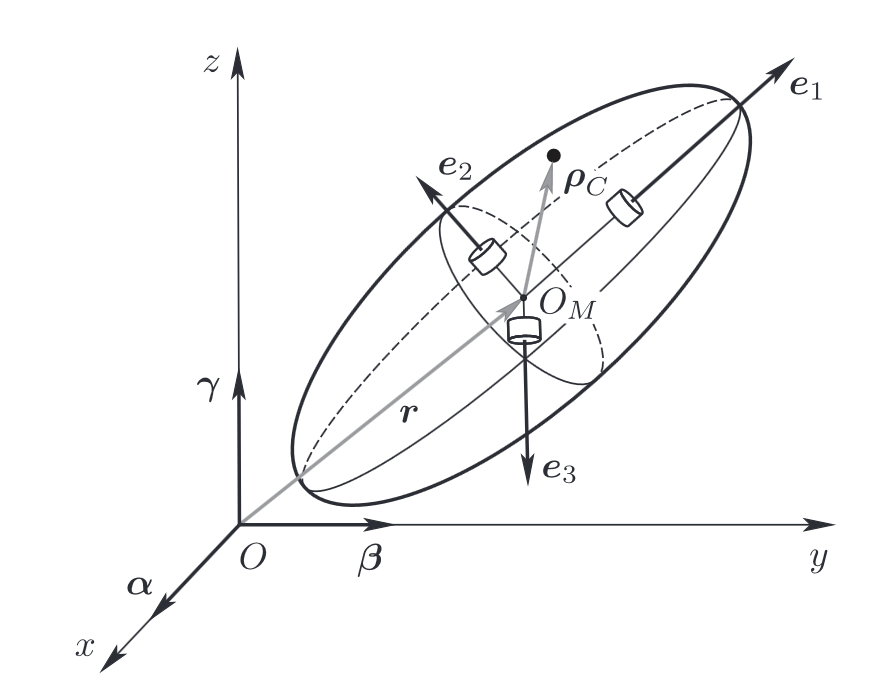
\includegraphics[width=0.4\linewidth]{BPR_Scheme.png}
		\caption{Схематическая модель безвинтового подводного робота с внутренними роторами, где $Oxyz$ --- неподвижная система координат, $O_M e_1 e_2 e_3$ --- подвижная система координат, $O_M$ --- геометрический центр эллипсоида, $\br = (x,y,z)$ --- радиус-вектор объекта, $\bbs \rho_C$ --- вектор центра масс системы в подвижной системе координат} \label{rotors}
	\end{center}
\end{figure}

Уравнения движения рассматриваемой системы записаны с помощью классических уравнений Кирхгофа:
 %\cite{Borisov_Mamaev}
\begin{gather}
\label{Kirchhoff}
\frac{d}{dt} \biggl( \frac{\partial T}{\partial \bV} \biggr) + {\bOm} \times \frac{\partial T}{\partial \bV}=0, \quad \frac{d}{dt}\biggl( \frac{\partial T}{\partial {\bOm}} \biggr) + {\bOm} \times \frac{\partial T}{\partial {\bOm}} + \bV \times \frac{\partial T}{\partial \bV} = 0 \nonumber
\end{gather}
где $\bV$ и ${\bOm}$ --- скорость центра оболочки и его угловая скорость, $T$ --- суммарная кинетическая энергия, состоящая из кинетической энергии оболочки, кинетической энергии жидкости и кинетической энергии каждого ротора.

Данные уравнения необходимо дополнить уравнениями эволюции переменных $\bigl( \br,\, {\bbQ} \bigr)$, которые описываются уравнениями Пуассона и кинематическими соотношениями следующего вида
\begin{gather}
\begin{gathered}
\dot{{\bal}} = {\bal} \times {\bOm},\quad \dot{{\bbe}} = {\bbe} \times {\bOm},\quad \dot{{\bga}} = {\bga} \times {\bOm}, \quad
\dot{\br} = {\bbQ}^T \bV.
\label{kinematics_abg}
\end{gathered}
\end{gather}
где ${\bal}$, ${\bbe}$, ${\bga}$ орты неподвижных осей $O x y z$, спроецированные на подвижные оси $e_1$, $e_2$, $e_3$, $\bbQ$ ортогональная матрица, состоящая из компонент векторов ${\bal}$, ${\bbe}$, ${\bga}$.
%\begin{gather*}
%\bbQ =\begin{pmatrix}
%\alpha _1 & \beta _1 & \gamma _1\\
%\alpha _2 & \beta _2 & \gamma _2\\
%\alpha _3 & \beta _3 & \gamma _3
%\end{pmatrix} 
%\label{eq.Qabg}
%\end{gather*}

%Обозначим через $m_s$ -- массу оболочки, ${\bm I}_s$ -- ее центральный тензор инерции, $\bLam = \diag(\bLam_1, \bLam_2) $
%%\begin{gather}
%%\bLam = \begin{pmatrix}
%%\bLam _1 & 0 \\
%%0 & \bLam _2
%%\end{pmatrix}\nonumber
%%\end{gather}
%-- матрицу коэффициентов присоединенных масс в системе $O_M e_1 e_2 e_3$, где $\bLam_1$ -- тензор присоединенных масс, $\bLam_2$ -- тензор присоединенных моментов инерции. Отметим, что в силу выбранных систем координат, тензоры $\bLam_1$ и $\bLam_2$ имеют диагональный вид: $\bLam_1=\diag(\lambda_1, \lambda_2, \lambda_3)$, $\bLam_2=\diag(\lambda_4, \lambda_5, \lambda_6)$. Тогда выражение для кинетической энергии оболочки примет вид
%\begin{gather}
%T_s = \frac{1}{2} m_s  \bigl( \bV,\, \bV \bigr) + \frac{1}{2} \bigl( {\bm I}_s {\bOm},\, {\bOm} \bigr),\nonumber
%\end{gather}
%а выражение кинетической энергии жидкости
%\begin{gather}
%T_f = \frac{1}{2} \bigl( \bLam_1 \bV,\, \bV \bigr) + \frac{1}{2} \bigl( {\bLam} _2 {\bOm},\, {\bOm} \bigr).\nonumber
%\end{gather}
%
%Обозначим через $m_R$ -- массу ротора, ${\bbI}_k$ -- центральный тензор инерции $k$-го ротора, записанный в системе координат $O_M e_1 e_2 e_3$, $\bn_k$ -- орт оси вращения $k$-го ротора неподвижный в системе $O_M e_1 e_2 e_3$, $\br_k$ -- радиус-вектор центра масс $k$-го ротора неподвижный в системе $O_M e_1 e_2 e_3$. Тогда кинетическая энергия $k$-го ротора примет вид
%\begin{gather}
%T_k = \frac{1}{2} m_R \bigl( \bV + {\bOm} \times \br_k, \bV + {\bOm} \times \br_k \bigr) + \frac{1}{2}\Bigl({\bm I}_k \bigl( {\bOm} + \omega_k \bn_k \bigr), {\bOm} + \omega_k \bn_k \Bigr).\nonumber
%\end{gather}

После подстановки кинетической энергии в уравнения Кирхгоффа уравнения движения принимают вид
\begin{gather}
\label{motion_eq}
\begin{split}
{\bbC} \dot{\bV} + {\bbB} \dot{{\bOm}} = & \bigl( {\bbC} \bV + {\bbB} {\bOm} \bigr) \times {\bOm},\\
{\bbB}^T \dot{\bV} + {\bbI} \dot{{\bOm}} + \dot{\bK}(t) = & \bigl( {\bbB}^T \bV + {\bbI} {\bOm} + \bK(t) \bigr) \times {\bOm} + \bigl( {\bbC} \bV + {\bbB} {\bOm} \bigr) \times \bV
\end{split}
\end{gather}
где $\bbI$ --- тензор инерции всей системы, вычисленный относительно геометрического центра оболочки, матрицы $\bbB$ и $\bbC$ зависят от распределения масс и формы оболочки, $\bK(t)$ --- вектор гиростатического момента. 
%Матрицы $\bbI$, $\bbB$, $\bbC$ имеют вид
%\begin{gather}
%{\bbI} = {\bLam}_2 + {\bbI}_s + \sum _{k=1}^3 {\bbI}_k + \frac{1}{2} m_R \sum _{k=1}^3 \bigl( \br_k^2{\bbE} - \br_k \otimes \br_k \bigr),\nonumber \\
%{\bbC} = m {\bbE} + {\bLam}_1 = \diag(c_1, \, c_2, \, c_3),\nonumber \\
%{\bbB} = m \begin{pmatrix}\nonumber
%0 & z_c & -y_c\\
%-z_c & 0 & x_c\\
%y_c & -x_c & 0
%\end{pmatrix},\nonumber \\
%m = m_s + 3 m_R,\nonumber \\
%\bK(t)=\sum \limits_{k=0}^3 i_k \omega_k (t)\bn_k. \nonumber
%\end{gather}
%где $x_c$, $y_c$, $z_c$ --- компоненты радиус-вектора $\bbs \rho_C$ центра масс системы, $\omega _k$ --- угловая скорость вращения k-го ротора, $ i_k $ --- осевой момент инерции k-го ротора.

Уравнения \eqref{motion_eq} можно записать в форме импульса и момента импульса:
\begin{gather}
\label{motion_ham}
\dot{\bP}= \bP \times {\bOm},\quad \dot{\bM} = \bM \times {\bOm} + \bP \times \bV,
\end{gather}
где $\bP = \dfrac{\partial T}{\partial \bV}$ и $\bM = \dfrac{\partial T}{\partial {\bOm}}$ имеют гидродинамический смысл и называются, соответственно, импульсивным моментом и импульсивной силой~\footfullcite{Borisov_Mamaev}. 

Уравнения \eqref{kinematics_abg} допускают шесть геометрических интегралов движения:
\begin{gather}
{\bal}^2={\bbe}^2={\bga}^2=1,\, \bigl({\bal},\, {\bbe} \bigr) = \bigl({\bal},\, {\bga} \bigr) = \bigl({\bbe},\, {\bga} \bigr) = 0.\nonumber
\end{gather}

Уравнения (\ref{motion_ham}) допускают еще шесть первых интегралов движения:
\begin{gather}
(\bP,\, {\bal}),\, (\bP,\, {\bbe}),\, (\bP,\, {\bga}),\, (\bM + \br \times \bP,\, {\bal}),\, (\bM + \br \times \bP,\, {\bbe}),\, (\bM + \br \times \bP,\, {\bga}) \label{integrals}
\end{gather}

В случае движения из состояния покоя первые интегралы \eqref{integrals} приобретают особенно простой вид: $ \bP = 0, \quad \bM = 0 $.
%\begin{gather}
%\bP = 0, \quad \bM = 0, \nonumber
%\end{gather}

Таким образом, при движении из состояния покоя система уравнений, описывающих эволюцию ориентации и траектории движения при заданном управлении, имет вид:
\begin{gather}
\begin{gathered}
\dot{{\bal}} = {\widetilde{\bbI} \bK(t)}  \times {\bal},\quad
\dot{{\bbe}} = {\widetilde{\bbI} \bK(t)}  \times {\bbe},\quad
\dot{{\bga}} = {\widetilde{\bbI} \bK(t)}  \times {\bga},\\
\dot{\br} =  {\bbQ}^T \bbC^{-1} \bbB \widetilde{\bbI} \bK(t),
\end{gathered}
\label{motion_eq_simple}
\end{gather}
где $\widetilde{\bbI} = \bigl(\bbI - \bbB^T \bbC^{-1} \bbB \bigr)^{-1}$.

В системе уравнений~\eqref{motion_eq_simple} вектор гиростатического момента $ \bK(t) $ является управляющим воздействием, так как зависит от угловых скоростей роторов: $ \bK(t)=\sum \limits_{k=0}^3 i_k \omega_k (t)\bn_k $.

%Решения системы уравнений \eqref{motion_eq_simple} относительно $\bK(t)$ позволяют находить управляющие воздействия $\omega_k (t)$ для движения вдоль заданной траектории.

Далее в главе полученная система исследована на управляемость с использованием теоремы Рашевского-Чжоу~\footfullcite{Rashevskyi_1938}. Показано, что для того, чтобы получить управляемый объект с формой оболочки в виде эллипсоида вращения с центром масс всей системы в геометрическом центре эллипсоида, необходимо внести асимметрию в форму. Это можно сделать, добавив к оболочке винтовые лопасти. Так объект будет представлять из себя трехлопастной винт.

%Для исследования управляемости представим систему уравнений движения в виде:
%\begin{gather*}
%\dot{\bq} = \bX_1 (\psi,\, \theta,\, \varphi) \Omega_1 + \bX_2 (\psi,\, \theta,\, \varphi) \Omega_2 + \bX_3 (\psi,\, \theta,\, \varphi) \Omega_3.
%\label{eq.zu123}
%\end{gather*}
%%где $\alpha_i$, $\beta_i$, $\gamma_i$ выражаются через углы Эйлера с помощью соотношений \eqref{eq.Qabg}, \eqref{eq.QEuler}.
%
%Согласно теореме Рашевского-Чжоу \footfullcite{Rashevskyi_1938}, если, в данном случае для 6-мерного пространства состояний, определитель матрицы, составленной из компонент шести векторных полей, не равен нулю, то данные векторные поля линейно независимы и система является управляемой.
%
%Построим следующие векторные поля:
%\begin{gather*}
%\begin{gathered}
%\bX_{1,2} = \left[ \bX_1,\, \bX_2\right],\quad \bX_{3,1} = \left[ \bX_3,\, \bX_1\right],\quad \bX_{2,3} = \left[ \bX_2,\, \bX_3\right], \\  
%\bX_{1,(2,3)} = \left[ \bX_1,\, \bX_{2,3}\right],\quad \bX_{2,(3,1)} = \left[ \bX_2,\, \bX_{3,1}\right], \quad \bX_{3,(1,2)} = \left[ \bX_3,\, \bX_{1,2}\right].\\
%\end{gathered}\label{eq.fieldsDeficit}
%\end{gather*}
%
%Выберем три набора векторных полей
%\begin{gather*}
%\begin{gathered}
%\Bigl( \bX_1,\, \bX_2,\,\bX_3,\,\bX_{1,2},\,\bX_{2,3},\,\bX_{2,(3,1)},\, \Bigr),\quad
%\Bigl( \bX_1,\, \bX_2,\,\bX_3,\,\bX_{2,3},\,\bX_{3,1},\,\bX_{3,(1,2)},\, \Bigr), \\
%\Bigl( \bX_1,\, \bX_2,\,\bX_3,\,\bX_{3,1},\,\bX_{1,2},\,\bX_{1,(2,3)},\, \Bigr).
%\end{gathered}\label{eq.sets}
%\end{gather*}
%
%Условия линейной зависимости векторных полей в указанных наборах имеют вид
%\begin{gather*}
%\begin{gathered}
%x_c(c_2 - c_3) = 0,\quad
%y_c(c_3-c_1) = 0, \quad
%z_c(c_1-c_2) = 0.
%\end{gathered}\label{eq.lin}
%\end{gather*}
%где $x_c$, $y_c$, $z_c$ --- компоненты радиус-вектора $\bbs \rho_C$ центра масс системы, $c_1$, $c_2$, $c_3$ --- компоненты матрицы $\bbC$, расположенные на главной диагонали.
%
%Таким образом, движение в идеальной жидкости однородной оболочки, имеющей форму эллипсоида, вполне управляемо с помощью вращения трех роторов, за исключением трех частных случаев:
%\begin{enumerate}
%	\item Система “ оболочка + роторы” уравновешена;
%	\item Оболочка имеет сферическую форму;
%	\item Оболочка имеет форму эллипсоида вращения, а центра масс всей системы	расположен на оси вращения.
%\end{enumerate}
%
%Следовательно, чтобы получить управляемый объект с формой оболочки в виде эллипсоида вращения с центром масс всей системы в геометрическом центре эллипсоида, необходимо внести асимметрию в форму. Это можно сделать добавив к оболочке винтовые лопасти. Так, объект будет представлять из себя трехлопастной винт.

Далее произведено моделирование траекторий движения при вращении роторов с постоянной скоростью с использованием полученной модели движения.





{\textbf{В третьей главе}} описана конструкция безвинтового подводного робота с внутреними роторами. 

Безвинтовой подводный робот является мобильным роботом в форме эллипсоида вращения с лопастями и представляет собой сборную конструкцию (рисунок \ref{constr_BPR}). Основой конструкции является оболочка, составленная из двух одинаковых половин 1, присоединенных друг к другу по экваториальной плоскости с помощью перегородки 2. К оболочке крепятся лопасти 3. Размер эллипсоида составляет 300 х 200 мм. 
%Толщина оболочки (3 мм) и применяемый материал обеспечивают необходимую прочность при погружении и перемещении робота. 
%Соединение полуоболочек и платформы обеспечивает герметичность внутренней полости.

\begin{figure}[h]
	\centering
	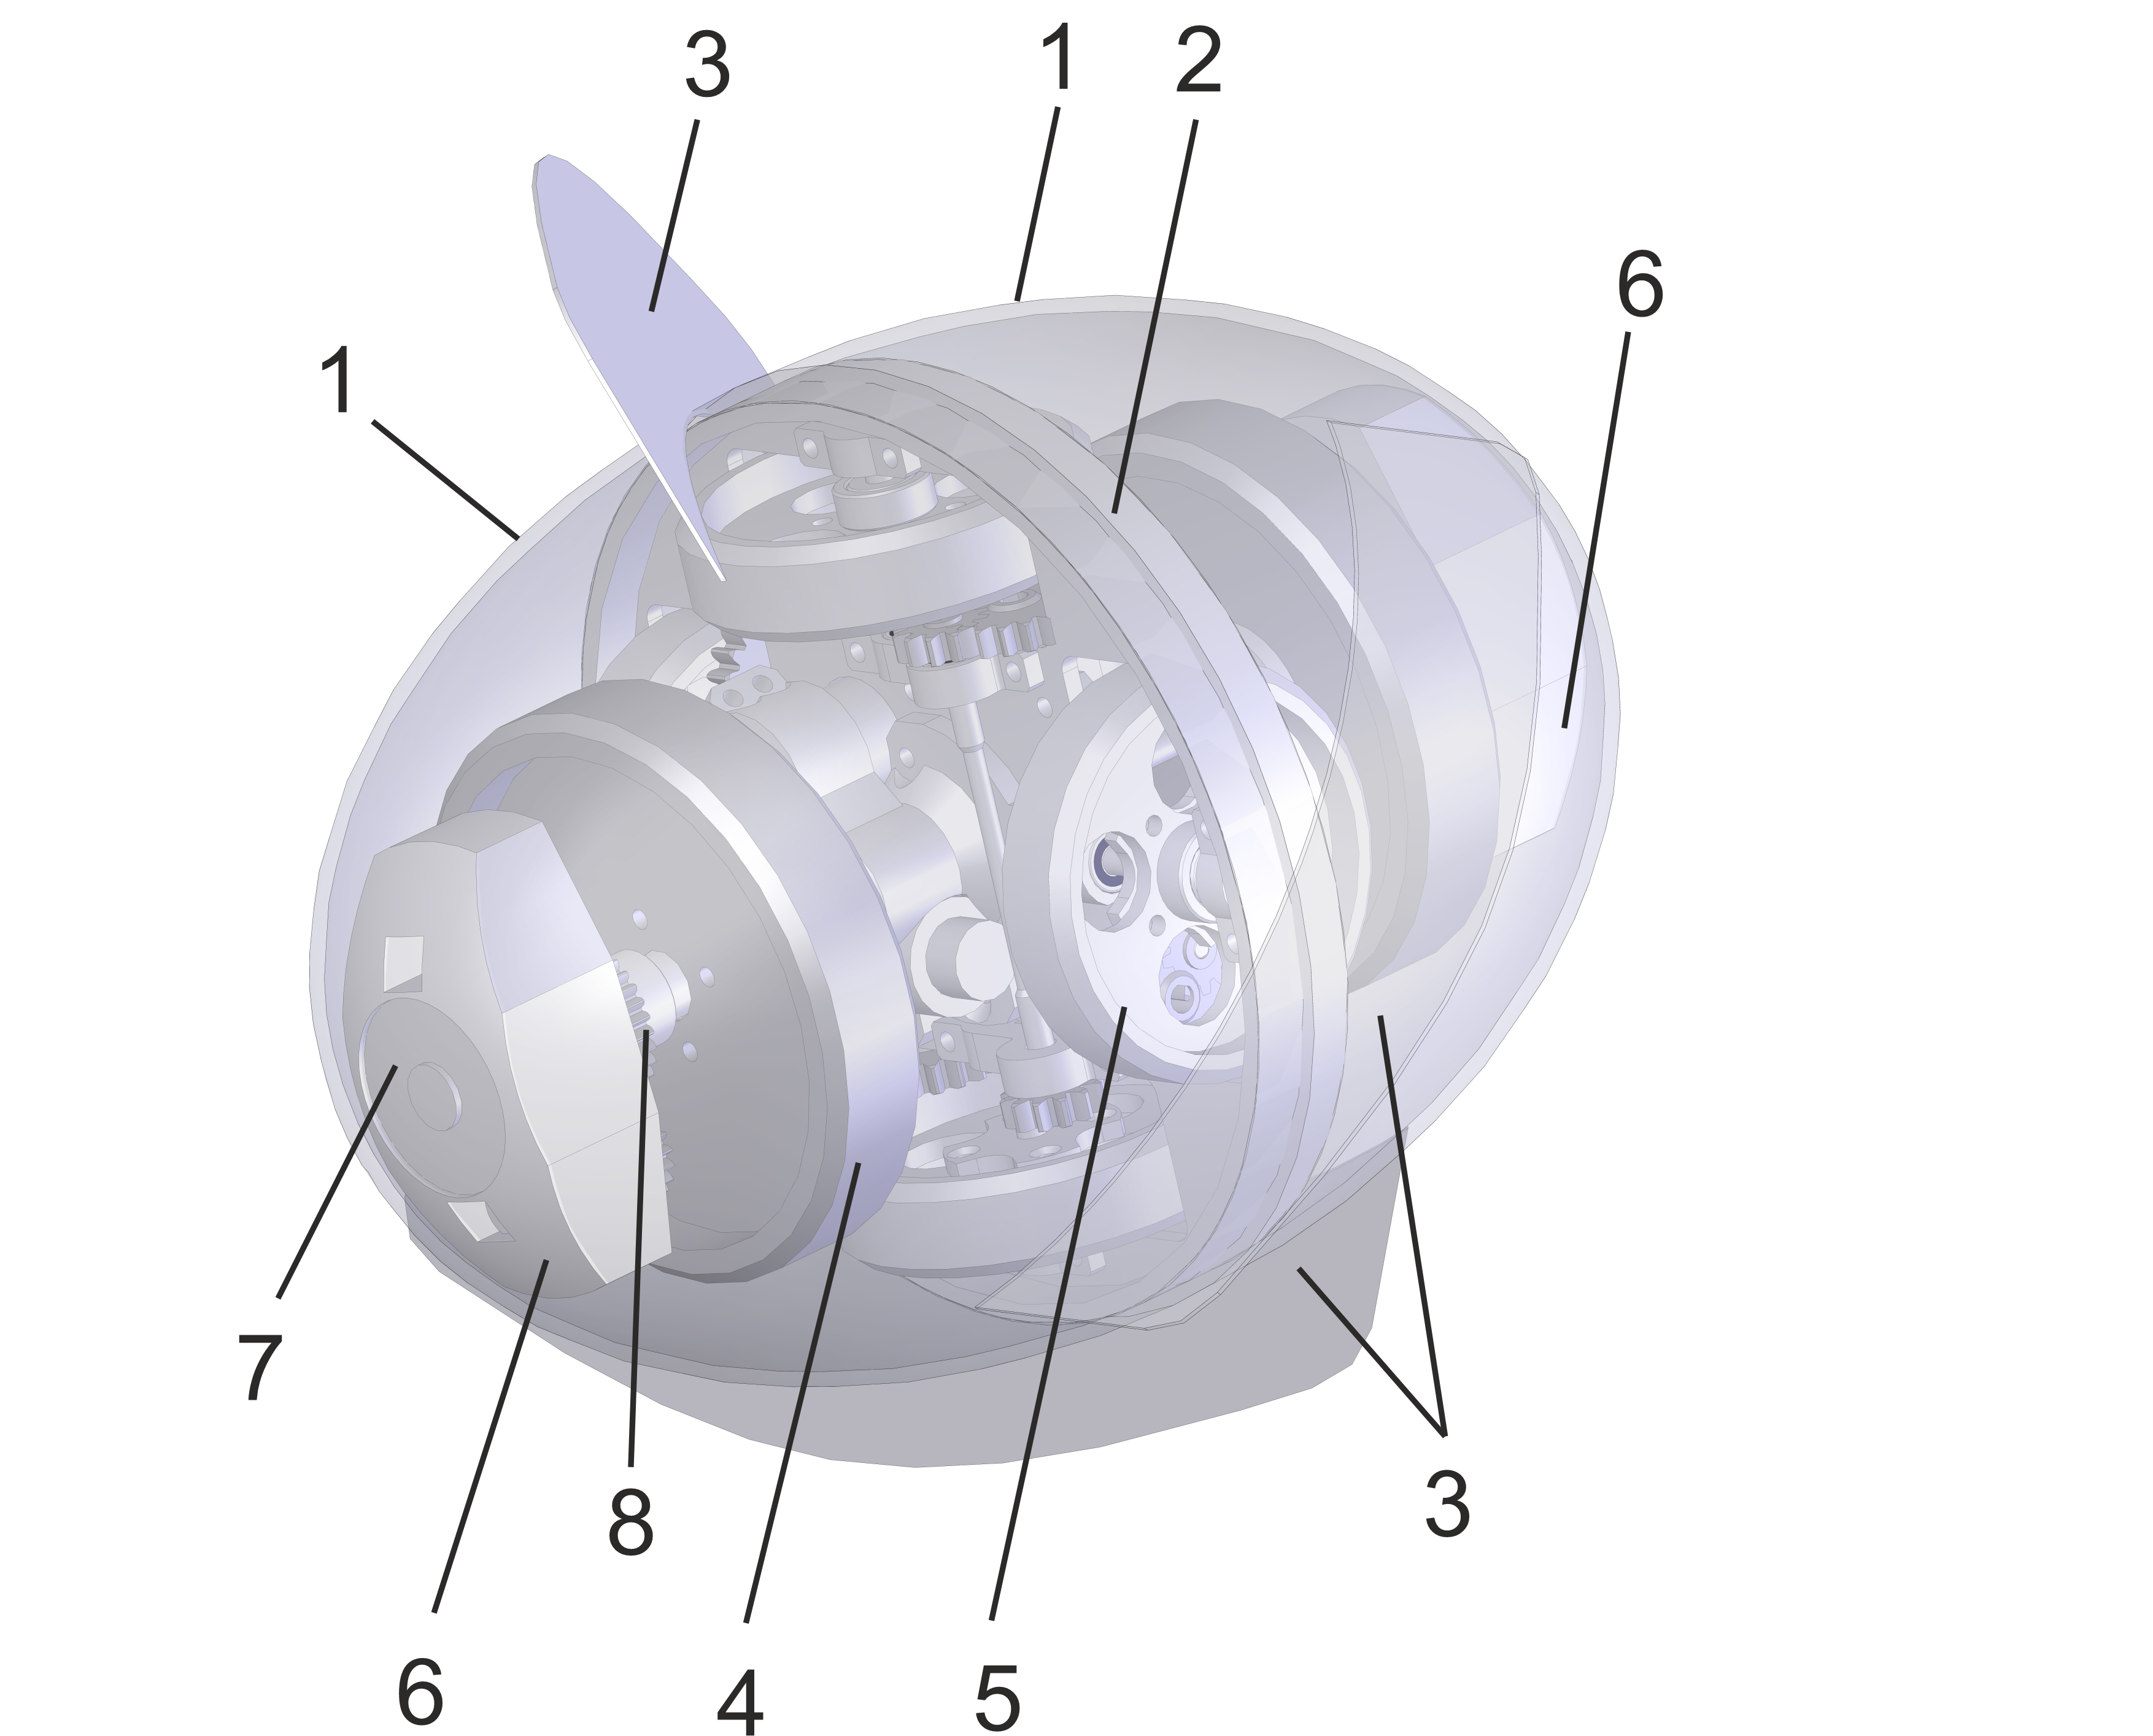
\includegraphics[width=0.4\linewidth]{BPR_ScrewModel.png}%
	\caption{Конструкция и корпусные элементы экспериментальной модели безвинтового подводного робота}
	\label{constr_BPR}
\end{figure}

%Размещение узлов на платформе выполнено таким образом, чтобы в максимальной степени обеспечить симметричное расположение масс относительно геометрического центра тела, а также по возможности обеспечить минимальное отклонение центра масс от геометрического.

Внутри корпуса робота три пары роторов установлены таким образом, что оси роторов расположены под углом $90^\circ$ по отношению друг к другу. Ось одной из пар роторов направлена вдоль оси вращения эллипсоида, а две другие пары расположены в экваториальной плоскости. 
%Обеспечение точного управляющего воздействия $\omega_k (t)$ осуществляется с помощью встроенных в приводы датчиков обратной связи (энкодеров). 
Система роторов подводного робота включает пару роторов большего размера 4 и две пары роторов меньшего размера 5. %Большие роторы 4 установлены симметрично относительно платформы 2 на одной общей оси. Две пары роторов меньшего размера 5, расположенны в экваториальной плоскости (по направлениям осей) и перпендикулярны друг другу. 
%Оси малых роторов выполнены отдельно для каждого маховика и установлены соосно на некотором расстоянии друг от друга.
%Малые роторы соединены кинематически попарно с помощью промежуточных (дополнительных) осей и зубчатых пар таким образом, что их вращение происходит также, как если бы они были на одной общей оси.
Для погружения робот оснащен механизмом регулировки плавучести 6. Модули плавучести имеют в своем составе поворотный пневмоцилиндр 7 с приводом 8. %Полости пневмоцилиндра --- воздушная и жидкостная имеют каналы, соединяющие их соответственно с внутренней полостью и внешней средой. %К выходному валу электродвигателя подсоединен редуктор с передаточным отношением 75:1, далее передача вращения от редуктора к пневмоцилиндру осуществляется с помощью пары шестерен с передаточным отношением 5.75:1.
Для придания роботу формы винтового тела к оболочке крепятся 3 лопасти. Полученное винтовое тело имеет диаметр винта 300 мм, угол наклона лопасти гребного винта к оси вращения эллипсоида --- 45$^{\circ}$. Фотографии робота в сборе и без половины оболочки представлены на рисунке~\ref{Photo_BPR}. 

\begin{figure}[h]
	\begin{minipage}[h]{0.5\linewidth}
		\center{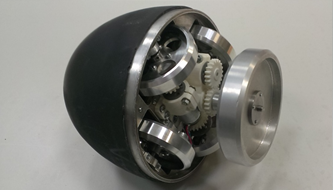
\includegraphics[width=1\linewidth]{Photo_BPR2.png} \\ а)}
	\end{minipage}
	\hfill
	\begin{minipage}[h]{0.5\linewidth}
		\center{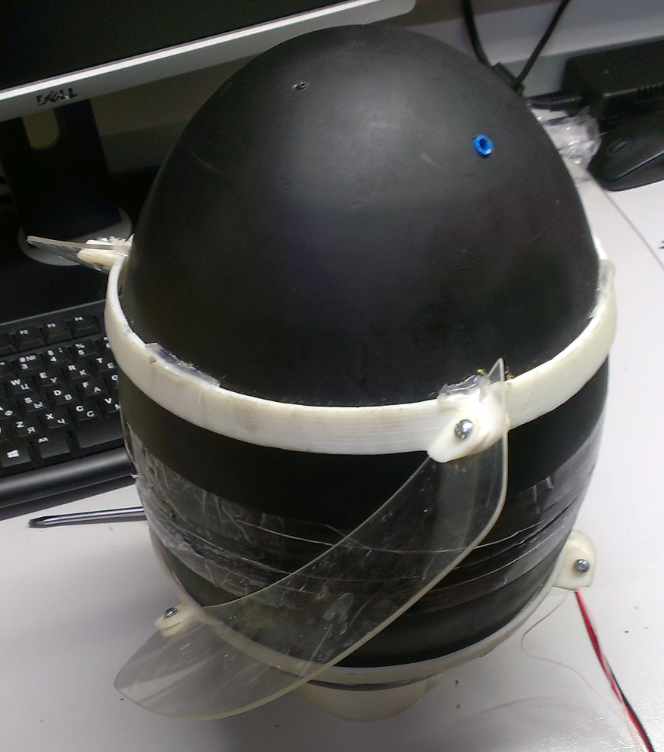
\includegraphics[width=0.5\linewidth]{BPR_Screw.png} \\ б)}
	\end{minipage}	
	\caption{Фотографии безвинтового подводного робота}
	\label{Photo_BPR}
\end{figure}

%\begin{figure}[h]
%	\centering
%	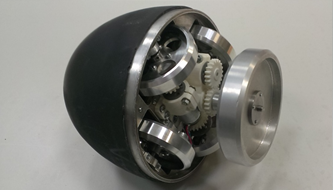
\includegraphics[width=0.9\linewidth]{Photo_BPR2.png}%
%	\caption{Фотографии безвинтового подводного робота}
%	\label{Photo_BPR}
%\end{figure}



%\begin{figure}[h]
%	\centering
%	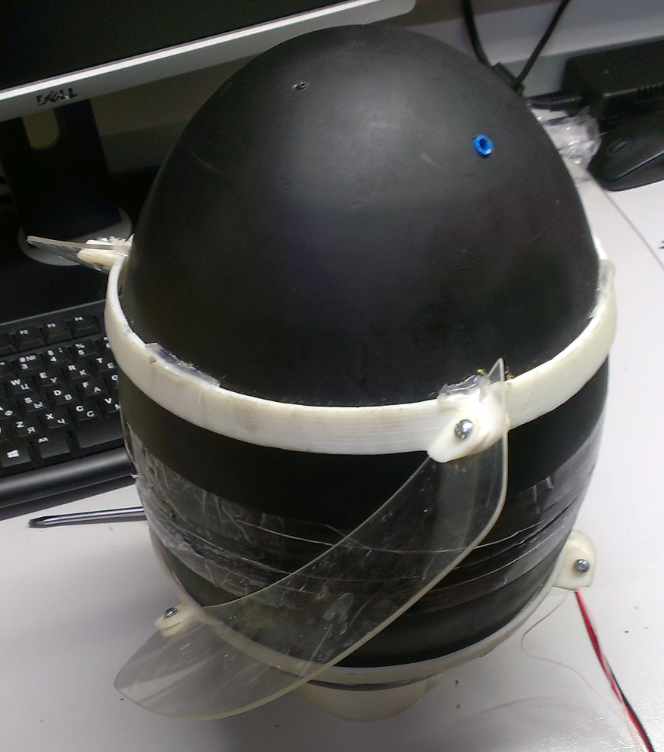
\includegraphics[width=0.4\linewidth]{BPR_Screw.png}%
%	\caption{Фотографии безвинтового подводного робота с лопастями}
%	\label{Photo_BPR_Screw}
%\end{figure}

%Структурная схема системы управления безвинтового подводного робота с внутренними роторами, представлена на рисунке \ref{str_scheme}.
%
%\begin{figure}[h!]
%	\begin{center}
%		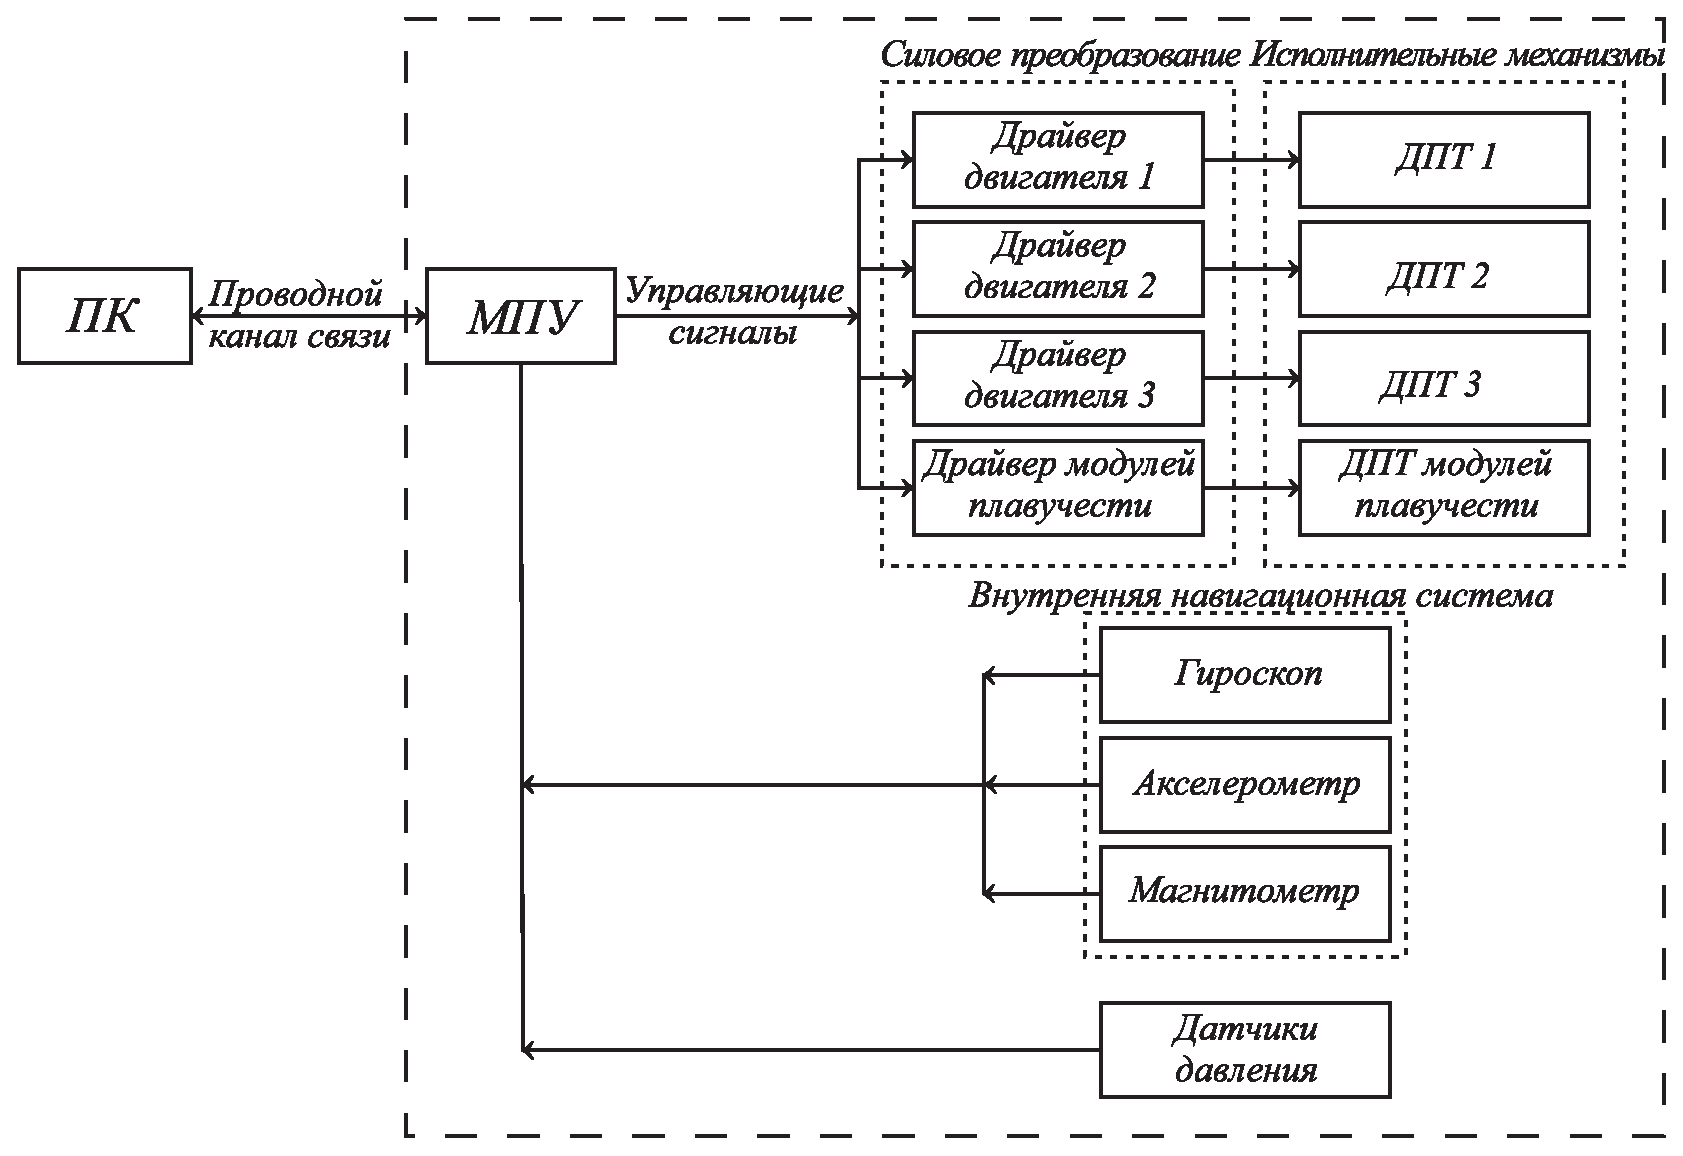
\includegraphics[width=0.8\linewidth]{StrSchemeBPR.eps}
%		\caption{Структурная схема системы управления подводным роботом} \label{str_scheme}
%	\end{center}
%\end{figure}


%Центральным элементом системы управления является микроконтроллер LPC1768FBD100 фирмы NXP. Данный микроконтроллер имеет ядро ARM Cortex-M3, работает на частоте до 100 МГц и содержит большой набор различной периферии. 
Управление роботом осуществляется с помощью микроконтроллера, который управляет двигателями постоянного тока, обрабатывает данные с датчиков обратной связи, а также может получать команды с программного обеспечения верхнего уровня.














В {\textbf{четвертой главе}} представлены результаты экспериментальных исследований движения в жидкости по типовым траекториям на основе математической модели движения безвинтового подводного робота. Эксперименты проводились в бассейне размерами 3 х 1.5 x 1.5 метра. При движении робота траектория отслеживалась с помощью системы захвата движения фирмы Contemplas, которая состоит из 4 камер.%, расположенных по периметру области съемки. Камеры предназначены для работы под водой. 

Цель экспериментов --- определение характера движения безвинтового подводного робота при различных управляющих воздействиях. 
%В качестве управляющих воздействий выступают гиростатические моменты роторов $K1, K2, K3$, возникающие при их вращении. 
Рассмотрены три серии экспериментов (по три эксперимента в каждой серии): вращение одной пары больших роторов, вращение одной пары малых роторов и одновременное вращение одной пары больших и одной пары малых роторов. В каждом эксперименте роторы разгонялись до максимальной скорости, которая поддерживалась постоянной в течение 3 секунд.

%Так как роторы 2 и 3 имеют одинаковые массо-геометрические характеристики и лежат в одной плоскости, их совместное вращение приведет к качественно аналогичному, результату, что и в случае их вращения по отдельности.

При вращении пары больших роторов траектории движения робота, полученные в эксперименте и при численном моделировании, представлены на рисунке~\ref{BPR_exp3}а. %Среднее значение перемещения при моделировании: $|\br_t| = 0.275$ м. Среднее значение перемещения в эксперименте: $|\br_{exp}| = 0.128$ м. 
%Cреднее значение перемещения расчитывалось по формуле: $ |\br| = \sqrt{(x_{st} - x_{fin})^2 + (y_{st} - y_{fin})^2 + (z_{st} - z_{fin})^2 )}$, где $ x_{st}, y_{st}, z_{st} $ --- координаты робота в момент начала движения в неподвижной системе координат, $ x_{fin}, y_{fin}, z_{fin} $ --- координаты робота в момент окончания движения в неподвижной системе координат.
%Среднее изменение координат геометрического центра робота ($\Delta x$, $\Delta y$, $\Delta z$) и изменение углов, определяющих положение, для трех экспериментов, и значения этих же параметров полученных с помощью теоретической модели представлены в таблице~\ref{tabExpBPR1}.
%\begin{table}[h]
%	\caption{Изменение положения и ориентации робота в теории и эксперименте} \label{tabExpBPR1}
%	\centering
%	\begin{tabular}{|c|c|c|c|c|c|c|c|}
%		\hline
%		& $\Delta x$, м & $\Delta y$, м & $\Delta z$, м & $|\br|$, м & $\Delta \theta$ & $\Delta \psi$ & $\Delta \varphi$ \\ \hline
%		Теория & $0.275$ & $0$ & $0$ & $0.275$ & $ 0^{\circ}$ & $ 0^{\circ}$ & $ 738.2^{\circ}$ \\ \hline
%		Эксперимент & $0.115$  & $0.010$ & $0.055$ & $0.128$ & $ 4^{\circ} $ & $ 10^{\circ} $ & $ 121^{\circ} $  \\
%		\hline
%	\end{tabular}
%\end{table}
%Здесь и далее $\theta$ --- угол дифферента --- угол между осью вращения эллипсоида и горизонтальной плоскостью; $\psi$ --- угол курса --- угол между осью вращения эллипсоида и вертикальной плоскостью (этот угол сходен с углом курса судна, но отсчитывается в соответствии с выбранной системой координат); $\varphi$ --- угол вращения --- угол, определяющий поворот робота вокруг оси вращения эллипсоида, $|\br|$ --- среднее значение перемещения, которое расчитывалось по формуле: $ |\br| = \sqrt{(x_{st} - x_{fin})^2 + (y_{st} - y_{fin})^2 + (z_{st} - z_{fin})^2 )}$, 
%\begin{gather*}
%|\br| = \sqrt{(x_{st} - x_{fin})^2 + (y_{st} - y_{fin})^2 + (z_{st} - z_{fin})^2 )},
%\end{gather*}
%где $ x_{st}, y_{st}, z_{st} $ --- координаты робота в момент начала движения в неподвижной системе координат, $ x_{fin}, y_{fin}, z_{fin} $ --- координаты робота в момент окончания движения в неподвижной системе координат.
При вращении одной пары малых роторов траектории движения робота, полученные в эксперименте и при численном моделировании, представлены на рисунке~\ref{BPR_exp3}б. %Среднее значение перемещения при моделировании: $|\br_t| = 0.005$ м. Среднее значение перемещения в эксперименте: $|\br_{exp}| = 0.087$ м.
%Среднее изменение координат геометрического центра робота и изменение углов, определяющих положение, для трех экспериментов, и значения этих же параметров полученных с помощью теоретической модели представлены в таблице~\ref{tabExpBPR2}.
%\begin{table}[h]
%	\caption{Изменение положения и ориентации робота в теории и эксперименте} \label{tabExpBPR2}
%	\centering
%	\begin{tabular}{|c|c|c|c|c|c|c|c|}
%		\hline
%		& $\Delta x$, м & $\Delta y$, м & $\Delta z$, м & $|\br|$, м & $\Delta \theta$ & $\Delta \psi$ & $\Delta \varphi$ \\ \hline
%		Теория & $0$ & $0.005$ & $0$ & $0.005$ & $ 35^{\circ}$ & $ 0^{\circ}$ & $ 0^{\circ}$ \\ \hline
%		Эксперимент & $0.054$  & $0.008$ & $0.068$ & $0.087$ & $ 61^{\circ} $ & $ 62^{\circ} $ & $ 10^{\circ} $  \\
%		\hline
%	\end{tabular}
%\end{table}
При вращении пары больших роторов и одной пары малых роторов траектории движения робота, полученные в эксперименте и при численном моделировании, представлены на рисунке~\ref{BPR_exp3}в. %Среднее значение перемещения при моделировании: $|\br_t| = 0.275$ м. Среднее значение перемещения в эксперименте: $|\br_{exp}| = 0.189$ м.
%Среднее изменение координат геометрического центра робота и изменение углов, определяющих положение, для трех экспериментов, и значения этих же параметров полученных с помощью теоретической модели представлены в таблице~\ref{tabExpBPR3}.
\begin{figure}[h]
	\begin{minipage}[h]{0.3\linewidth}
		\center{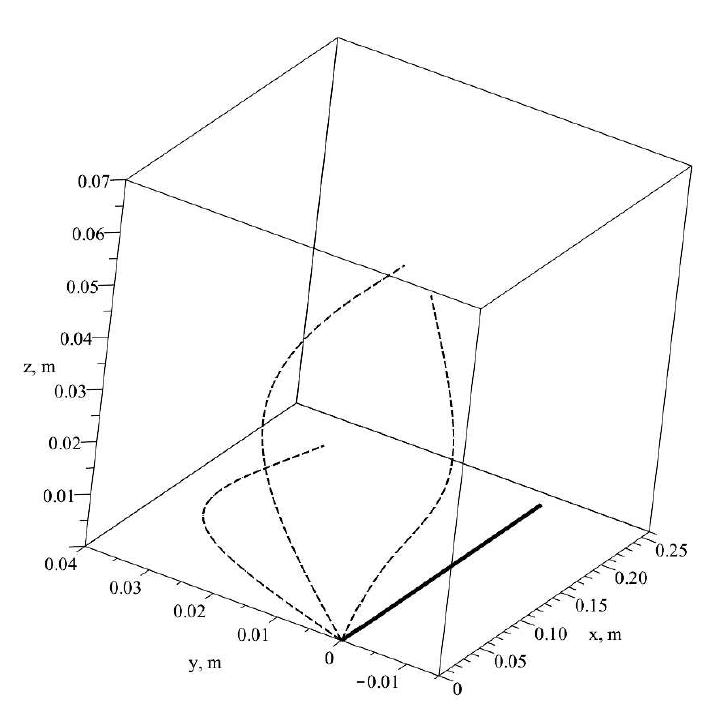
\includegraphics[width=0.9\linewidth]{Exp_BPR_1.png} \\ а)}
	\end{minipage}
	\hfill
	\begin{minipage}[h]{0.3\linewidth}
		\center{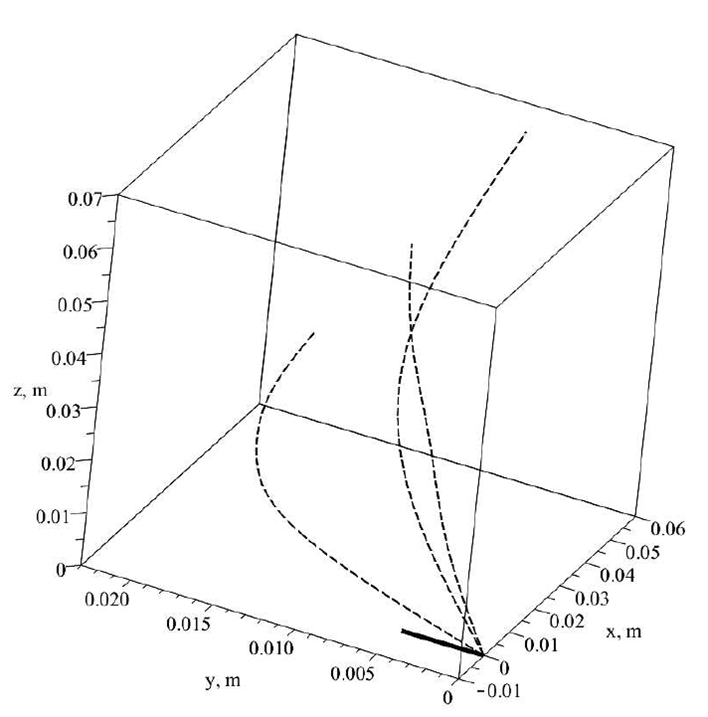
\includegraphics[width=0.9\linewidth]{Exp_BPR_2.png} \\ б)}
	\end{minipage}
	\hfill
	\begin{minipage}[h]{0.3\linewidth}
		\center{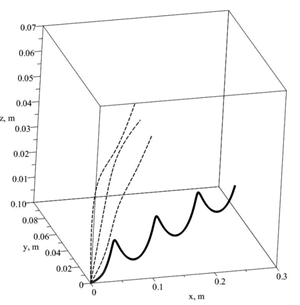
\includegraphics[width=0.9\linewidth]{Exp_BPR_3.png} \\ в)}
	\end{minipage}
	\caption{Траектории движения безвинтового подводного робота при а)~$\bK=(2i_1\omega_{max},  0,  0)$, б)~$\bK=( 0,  2i_2\omega_{max}, 0 )$, в)~$\bK=(2i_1\omega_{max},  0,  0)$}
	\label{BPR_exp3}
\end{figure}
%\begin{table}[h]
%	\caption{Изменение положения и ориентации робота в теории и эксперименте} \label{tabExpBPR3}
%	\centering
%	\begin{tabular}{|c|c|c|c|c|c|c|c|}
%		\hline
%		& $\Delta x$, м & $\Delta y$, м & $\Delta z$, м & $|\br|$, м & $\Delta \theta$ & $\Delta \psi$ & $\Delta \varphi$ \\ \hline
%		Теория & $0.275$ & $0$ & $0$ & $0.275$ & $ 35^{\circ}$ & $ 0^{\circ}$ & $ 738.2^{\circ}$ \\ \hline
%		Эксперимент & $0.106$  & $0.050$ & $0.053$ & $0.189$ & $ 17^{\circ} $ & $ 92^{\circ} $ & $ 51^{\circ} $  \\
%		\hline
%	\end{tabular}
%\end{table}

%Отметим, что в первых двух случаях управляющих воздействий в рамках теоретической модели робот движется прямолинейно не изменяя своей ориентации. При проведении экспериментов такого движения добиться не удается.
%Так же перемещение безвинтового подводного робота на практике меньше, чем в теории. 
%Более того в эксперименте при управляющем воздействии $\bK=\begin{pmatrix} 0,  2i_2\omega_{max}, 0 \end{pmatrix}$ движение робота происходит вдоль оси симметрии винтового тела (вдоль большей оси эллипсоида), а в теории робот движется перпендикулярно ей. 

Анализируя отклонения и характер движения безвинтового подводного робота в экспериментах, можно сделать следующие выводы:

\begin{enumerate}
	\item	Управляемое движение безвинтового подводного робота на практике продолжается до тех пор, пока обеспечивается ускоренное вращение роторов. Однако технически максимальная угловая скорость вращения роторов ограничена, и после ее достижения робот продолжает движение по инерции.
	%\item Разгон маховиков до максимальной скорости занимает определенное время (разгон большего маховика --- $t=0.9$ секунды, разгон малого маховика --- $t=0.7$ секунды), что не учитывается в теоретической модели и вносит свой вклад в траекторию движения безвинтового подводного робота.
	\item	Движение безвинтового подводного робота сопровождается образованием вихревых структур, что подтверждается данными, полученными с использованием системы визуализации потоков. %(PIV --- Particle Image Velocimetry). 	
	\item Математическая модель движения записана в рамках теории идеальной жидкости без учета вязкого сопротивления, что вносит несоответствия между теоретической и наблюдаемой в экспериментах траекториями движения.
	\item Подобную схему и алгоритмы управления в качестве практического применения можно использовать для реализации различных маневров (например, разворот на месте) в управлении подводными роботами.
	\item Модель качественно описывает движение, но на количественное согласование влияет точность определения большого количества параметров. Движение возможно, однако его эффективность невысока.
	
\end{enumerate}

Учитывая полученные результаты, для проведения дальнейшего исследования разработана вторая модель водного робота с внутренним ротором со следующими условиями:

\begin{enumerate}
	\item Использование модели движения, учитывающей вязкое сопротивление жидкости.
	%, так как вязкие эффекты существенно влияют на траекторию движения. 
	Для упрощения расчетов рассмотрим плоско-параллельное движение по поверхности жидкости.
	
	\item Использование ассиметричной формы оболочки робота. При движении с образованием вихревых структур необходимо выбрать такую форму оболочки робота, для которой образование вихрей не будет препятствовать движению. Такой формой может быть оболочка с острой кромкой, например, в виде симметричного профиля крыла Жуковского либо симметричного профиля крыла классификации NACA.
	
	\item Использование периодического управления. Движение робота происходит при ускоренном вращении роторов, а чтобы его обеспечить, необходимо периодически изменять направление вращения ротора. 
	
\end{enumerate}






В {\textbf{пятой главе}} описана конструкция безвинтового надводного робота с оболочкой, имеющей форму симметричного профиля с острой кромкой.

Робот представляет собой полый объект, в продольном сечении имеющий форму профиля крыла NACA 0040 (см. рисунок \ref{Photo_NACA}а) длиной 340 мм, шириной 134 мм. Высота робота 80 мм. 
%Форма профиля крыла NACA 0040 задается функцией $ y = \frac{T}{0.2}(a_0\sqrt{x} + a_1x + a_2x^2 + a_3x^3 + a_4x^4 $, где $a_0=0.2969$, $a_1=-0.126$, $a_2=-0.3516$, $a_3=0.2843$, $a_4=-0.1036$, $T=0.4$. Точки контура профиля были рассчитаны в среде Matlab и импортированы в среду разработки Компас-3Д.	



\begin{figure}[h]
	\begin{minipage}[h]{0.5\linewidth}
		\center{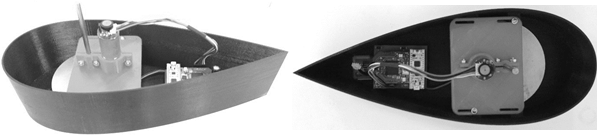
\includegraphics[width=1\linewidth]{Photo_NACA.png} }
	\end{minipage}
	\hfill
	\begin{minipage}[h]{0.5\linewidth}
		\center{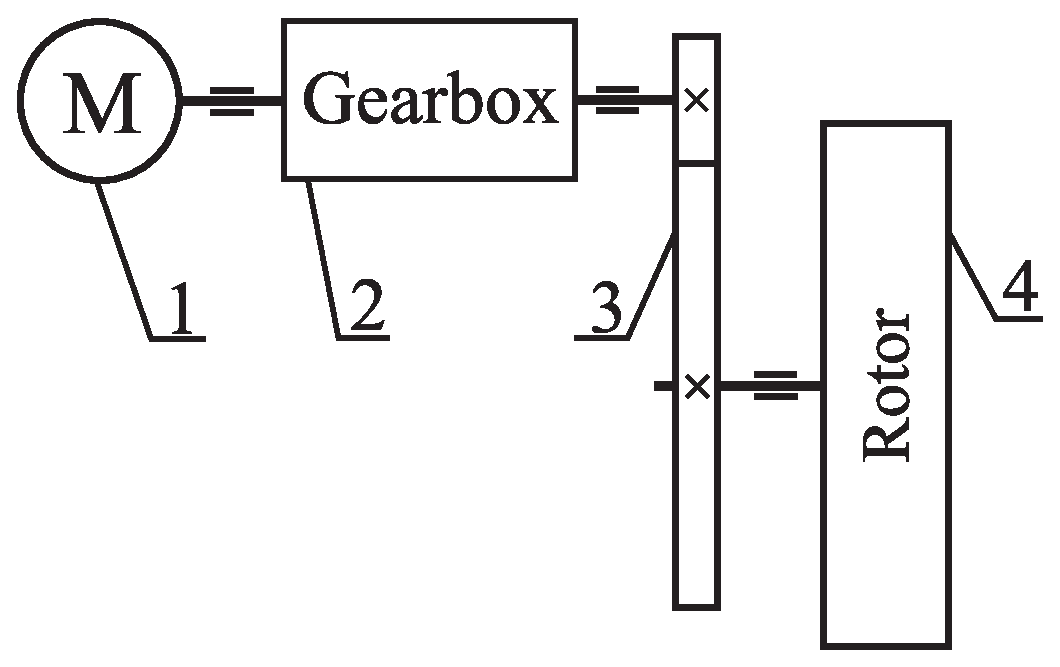
\includegraphics[width=0.6\linewidth]{Kinematic_Scheme2.eps} }
	\end{minipage}
	
	\begin{minipage}[h]{0.5\linewidth}
		\center{а)}
	\end{minipage}
	\hfill
	\begin{minipage}[h]{0.5\linewidth}
		\center{б)}
	\end{minipage}
	\caption{а) Безвинтовой надводный робот с острой кромкой. б) Кинематическая схема передачи вращения от двигателя к ротору}
	\label{Photo_NACA}
\end{figure}

%Корпус изготовлен на 3Д-принтере из PLA-пластика с толщиной стенки в 2 мм. 
Внутри оболочки робота закреплен ротор 4 с двигателем 1 таким образом, что центр масс всей системы находится максимально близко к нижней грани робота. Для передачи вращения с двигателя к ротору использовался редуктор 2 и пара шестерен 3. Кинематическая схема передачи вращения от двигателя к ротору представлена на рисунке~\ref{Photo_NACA}б. Внутри также располагается элемент питания и плата с микроконтроллером, управляющим вращением двигателя постоянного тока. %Микроконтроллер расположен на отладочной плате Nucleo-32 от фирмы STMicroelectronics.

%В качестве модуля питания используется литий-полимерная (Li-Po) аккумуляторная батарея фирмы nVision с номинальным напряжением 7.4 Вольта, емкостью 450 мАЧ и максимальным выходным током до 13.5 Ампер.

%Данная плата имеет 30 выводов; содержит программатор ST-Link, с помощью которого можно программировать микроконтроллер подключив плату к персональномук компьютеру по USB-кабелю; имеет необходимую обвязку из электронных компонентов, необходимых для стабильной работы микроконтроллера, кнопку сброса микроконтроллера и 3 светодиода: один пользовательский светодиод, светодиод, отображающий подачу питания на плату и светодиод сигнализирующий о передаче данных по USB-интерфейсу; может питаться как от USB-кабеля, так и от внешнего напряжения 7--15 Вольт. Данная плата поддерживает среду разработки ARM mbed, которая позволяет разрабатывать программное обеспечение для микроконтроллера используя онлайн среду программирования. 

Для управления безвинтовым надводным роботом с острой кромкой была разработана система управления, структурная схема которой представлена на рисунке~\ref{ControlSystem}. На схеме $ \omega_{set} $ -- заданная скорость вращения ротора. Блок регулятора скорости представляет собой ПИД-регулятор, который обеспечивает поддержание значения заданной скорости. На выходе данного блока получаем ШИМ-сигнал необходимой скважности. Коэффициенты ПИД-регулятора подобраны экспериментально. Далее ШИМ-сигнал подается на драйвер двигателя постоянного тока, который его усиливает до необходимого напряжения и подает на обмотки двигателя. 
%В данной работе используется драйвер двигателя постоянного тока VNH3SP30 фирмы STMicroelectronics. 
На валу двигателя располагается датчик положения вала (энкодер), с помощью которого измеряется угол поворота вала двигателя $ \varphi $, с помощью которого можно рассчитать значение $ \hat{\omega}_{set} $ -- фактическую скорость вращения ротора. Полученное значение $ \hat{\omega}_{set} $ учитывается блоком регулятора скорости при расчете управляющих сигналов, идущих на двигатель. 
%При вращении ротора данный алгоритм должен выполняться через промежутки времени $ \Delta t \rightarrow 0 $. Выбранный микроконтроллер имеет максимальную частоту работы 72 МГц, что позволяет выбрать $ \Delta t = 1 $ мс. Значение $ \Delta t $ выбрано экспериментально.

\begin{figure}[!h]
	\centering
	\includegraphics[width=0.65\linewidth]{ControlSystem.eps}
	\caption{Структурная схема системы управления безвинтового надводного робота с острой кромкой}
	\label{ControlSystem}
\end{figure}















В {\textbf{шестой главе}} представлены результаты разработки математической модели движения в жидкости безвинтового надводного робота с острой кромкой.

Для описания движения робота введем две системы координат: неподвижную $Oxy$ и подвижную $Cx_1x_2$, жестко связанную с телом (см. рисунок~\ref{fig.coords}), точка $C$ совпадает с центром масс системы. 
%Будем считать, что ось $Cx_1$ подвижной системы координат совпадает с осью симметрии профиля, а точка $C$ совпадает с центром масс системы <<профиль + ротор>>. 
Положение подвижной системы координат относительно неподвижной будем задавать с помощью радиус-вектора $\bm r = (x,\, y)$ точки $C$, а ее ориентацию углом $\alpha$. %между положительными направлениями осей $Ox$ и $Cx_1$, отсчитываемым от оси $Ox$.

\begin{figure}[h!]
	\centering
	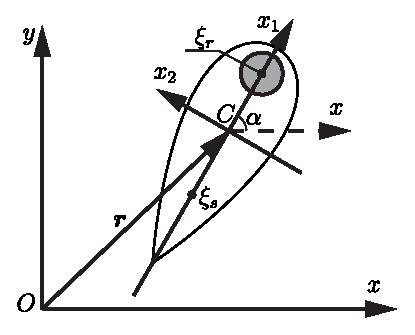
\includegraphics[width=0.3\linewidth]{coords.eps}
	\caption{$Oxy$ --- неподвижная система координат, $Cx_1x_2$ --- подвижная система координат}\label{fig.coords}
\end{figure}

Справедливы следующие кинематические соотношения:
\begin{gather}
\begin{gathered}
\dot{x} = v_1 \cos\alpha - v_2 \sin\alpha,\quad \dot{y} = v_1 \sin\alpha + v_2 \cos\alpha,\quad \dot{\alpha} = \omega,
\end{gathered}\label{eq.kinem}
\end{gather}
где $v_1$, $v_2$ --- проекции вектора поступательной скорости точки $C$ на подвижные оси, $\omega$ --- угловая скорость тела.

Для описания движения мы воспользуемся уравнениями Ньютона-Эйлера при дополнительном предположении, что силы и момент сил, действующие на тело, зависят только от его скоростей и ускорений: %Так в подвижных осях, жестко связанных с телом, уравнения движения имеют вид:
\begin{gather}
\begin{gathered}
m \dot{v}_1 = m v_2 \omega + f_1 (v_1,\, v_2,\, \omega,\, \dot{v}_1,\, \dot{v}_2,\, \dot \omega),\
m \dot{v}_2 = -m v_1 \omega + f_2 (v_1,\, v_2,\, \omega,\, \dot{v}_1,\, \dot{v}_2,\, \dot \omega),\\
I \dot{\omega} = g (v_1,\, v_2,\, \omega,\, \dot{v}_1,\, \dot{v}_2,\, \dot \omega),
\end{gathered}\label{eq.NE}
\end{gather}
где $m$, $I$ --- масса и момент инерции робота соответственно, $f_1$, $f_2$ --- проекции силы реакции жидкости на подвижные оси, связанные с телом, $g$ --- момент силы реакции жидкости. 

Для определения вида $ f_1 $, $ f_2 $ и $ g $ воспользуемся уравнениями Кирхгофа, дополненные слагаемыми, описывающими вязкое сопротивление:% \cite{Borisov_et_al_2016}:
\begin{equation}
\begin{gathered}
\der{}{t} \pder{T}{v_1} = \omega \pder{T}{v_2} - c_1 v_1 |v_1|,\quad \der{}{t} \pder{T}{v_2} = - \omega \pder{T}{v_1} - c_2 v_2 |v_2|,\\
\der{}{t} \pder{T}{\omega} = v_2 \pder{T}{v_1} - v_1 \pder{T}{v_2} - c_3 \omega |\omega|,
\end{gathered}\label{eq.kirchhoff}
\end{equation}
где $c_1,\,c_2,\,c_3$ --- коэффициенты вязкого сопротивления, $ T $ --- кинетическая энергия системы, состоящая из кинетической энергии оболочки, кинетической энергии жидкости и кинетической энергии ротора.

%Кинетическая энергия системы с точностью до некоторой функции времени имеет вид
%\begin{gather}
%T = \frac{1}{2}(m + \lambda_{11}) v_1^2 + \frac{1}{2}(m + \lambda_{22}) v_2^2 + \frac{1}{2} (I + \lambda_{33}) \omega^2 + \lambda_{23} v_2\omega + \omega k(t),\label{eq.T}\\
%\begin{gathered}
%m = m_s + m_r,\quad
%I = I_s + m_s \xi_s^2 + I_r + m_r \xi_r^2,\quad k(t) = I_r \Omega(t),
%\end{gathered}\notag
%\end{gather}
%где $m_s$, $I_s$ --- масса и центральный момент инерции корпуса робота, $m_r$, $I_r$ --- масса и центральный момент инерции ротора, $\xi_s$ --- положение центра масс корпуса робота, $\xi_r$ --- положение центра масс ротора, $\Omega(t)$ --- угловая скорость ротора, $\lambda_{11}$, $\lambda_{22}$ --- присоединенные массы, $\lambda_{33}$ --- присоединенный момент инерции, $\lambda_{23}$ --- коэффициент, возникающий вследствие смещения центра давления относительно центра масс.

После подстановки кинетической энергии в уравнение \eqref{eq.kirchhoff}, полная система уравнений рассматриваемой системы может быть записана в следующей форме:
\begin{subequations}\label{eq.fullEqs}
	\begin{equation}
	\begin{split}\label{eq.dyn}
	(m + \lambda_{11}) \dot{v}_1 = {} & {} (m + \lambda_{22}) v_2 \omega + \lambda_{23}\omega^2 - c_1 v_1 |v_1|,\\
	(m + \lambda_{22}) \dot{v}_2 + \lambda_{23} \dot{\omega} = {} & {} - (m + \lambda_{11}) v_1 \omega - c_2 v_2 |v_2|,\\
	\lambda_{23}\dot{v}_2 + (I + \lambda_{33}) \dot{\omega} = {} & {} (\lambda_{11} - \lambda_{22}) v_1 v_2 - \lambda_{23} v_1\omega - c_3 \omega |\omega| - \dot{k}(t),
	\end{split}
	\end{equation}
	\begin{equation}
	\dot{x} = v_1 \cos\alpha - v_2 \sin\alpha,\quad \dot{y} = v_1 \sin\alpha + v_2 \cos\alpha,\quad \dot{\alpha} = \omega.
	\end{equation}
\end{subequations}
где $\lambda_{11}$, $\lambda_{22}$ --- присоединенные массы, $\lambda_{33}$ --- присоединенный момент инерции, $\lambda_{23}$ --- коэффициент, возникающий вследствие смещения центра давления относительно центра масс; $ k(t) $ --- гиростатический момент ротора.

Сравнивая уравнения \eqref{eq.dyn} с уравнениями Ньютона-Эйлера \eqref{eq.NE}, запишем выражения для сил $f_1$, $f_2$ и момента $g$:
\begin{gather}
\begin{gathered}\label{eq.forceTorque}
f_1 = - \lambda_{11}\dot{v}_1 + \lambda_{22} v_2 \omega + \lambda_{23}\omega^2 - c_1 v_1 |v_1|, \\
f_2 = - \lambda_{22} \dot{v}_2 - \lambda_{23} \dot{\omega} - \lambda_{11} v_1 \omega - c_2 v_2 |v_2|,\\
g = -\lambda_{23}\dot{v}_2 - \lambda_{33} \dot{\omega} + (\lambda_{11} - \lambda_{22}) v_1 v_2 - \lambda_{23} v_1\omega - c_3 \omega |\omega| - \dot{k}(t),
\end{gathered}
\end{gather}
где коэффициенты $\lambda_{ij}$ и $c_i$ подлежат определению, а $\dot{k}(t)$ является управляющим воздействием. Для определения коэффициентов, входящих в эти выражения, мы воспользуемся подходом, основанным на численном решении уравнений Навье-Стокса, используя экспериментальные данные.

Анализ разработанной модели позволит сформировать управляющие воздействия. Зададим управление движением ротора $\Omega(t)$  при помощи кусочно-непрерывной периодической функции, представленной на рисунке~\ref{ControlAction}а.

%\begin{gather}\label{omegaRotorGeneral}
%\Omega(t) = \begin{cases}
%\Omega_1(t), & t \in \left[ nT,\, nT + t_1 \right],\\
%\Omega_2(t), & t \in \left[ nT + t_1,\, nT + t_1 + t_2 \right],\\
%\Omega_3(t), & t \in \left[ nT + t_1 + t_2,\, nT + t_1 + t_2 + t_3 \right],\\
%\Omega_4(t), & t \in \left[ nT + t_1 + t_2 + t_3,\, nT + t_1 + t_2 + t_3 + t_4 \right]
%\end{cases}\\
%\Omega_1(t) = \omega_1,\quad \Omega_2(t) = \dfrac{(\omega_2 - \omega_1)(t-nT)}{t_2} - \dfrac{(\omega_2 - \omega_1)(t_1+t_2)}{t_2} + \omega_2, \notag\\
%\Omega_3(t) = \omega_2,\quad \Omega_4(t) = \dfrac{(\omega_1 - \omega_2)(t-nT)}{t_4} - \dfrac{(\omega_1 - \omega_2)(t_1+t_2+t_3+t_4)}{t_4} + \omega_1,\notag
%\end{gather}
%где $n \in \mathbb{N}$, $T$ --- период управляющего воздействия; $t_1, t_3$ --- задают интервалы времени с постоянными угловыми скоростями вращения ротора $\omega_1$, $\omega_2$ соответственно, $t_2$, $t_4$ --- интервалы равноускоренного вращения ротора. Графически данная зависимость приведена на рис.~\ref{ControlAction}.

\begin{figure}[!ht]
	\begin{minipage}[h]{0.3\linewidth}
		\center{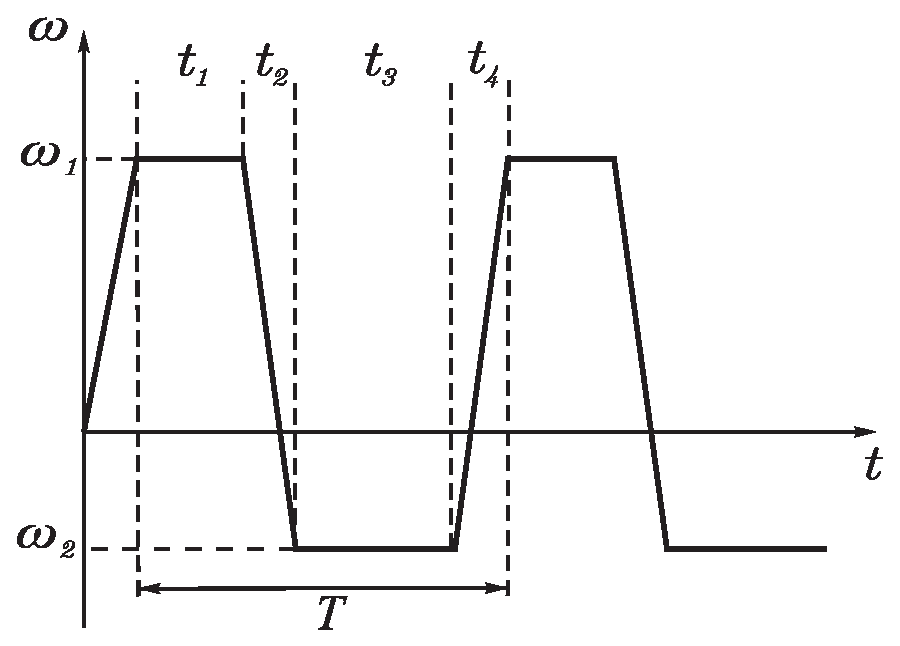
\includegraphics[height=0.7\linewidth]{ControlAction.eps} \\ }
	\end{minipage}
	\hfill
	\begin{minipage}[h]{0.7\linewidth}
		\center{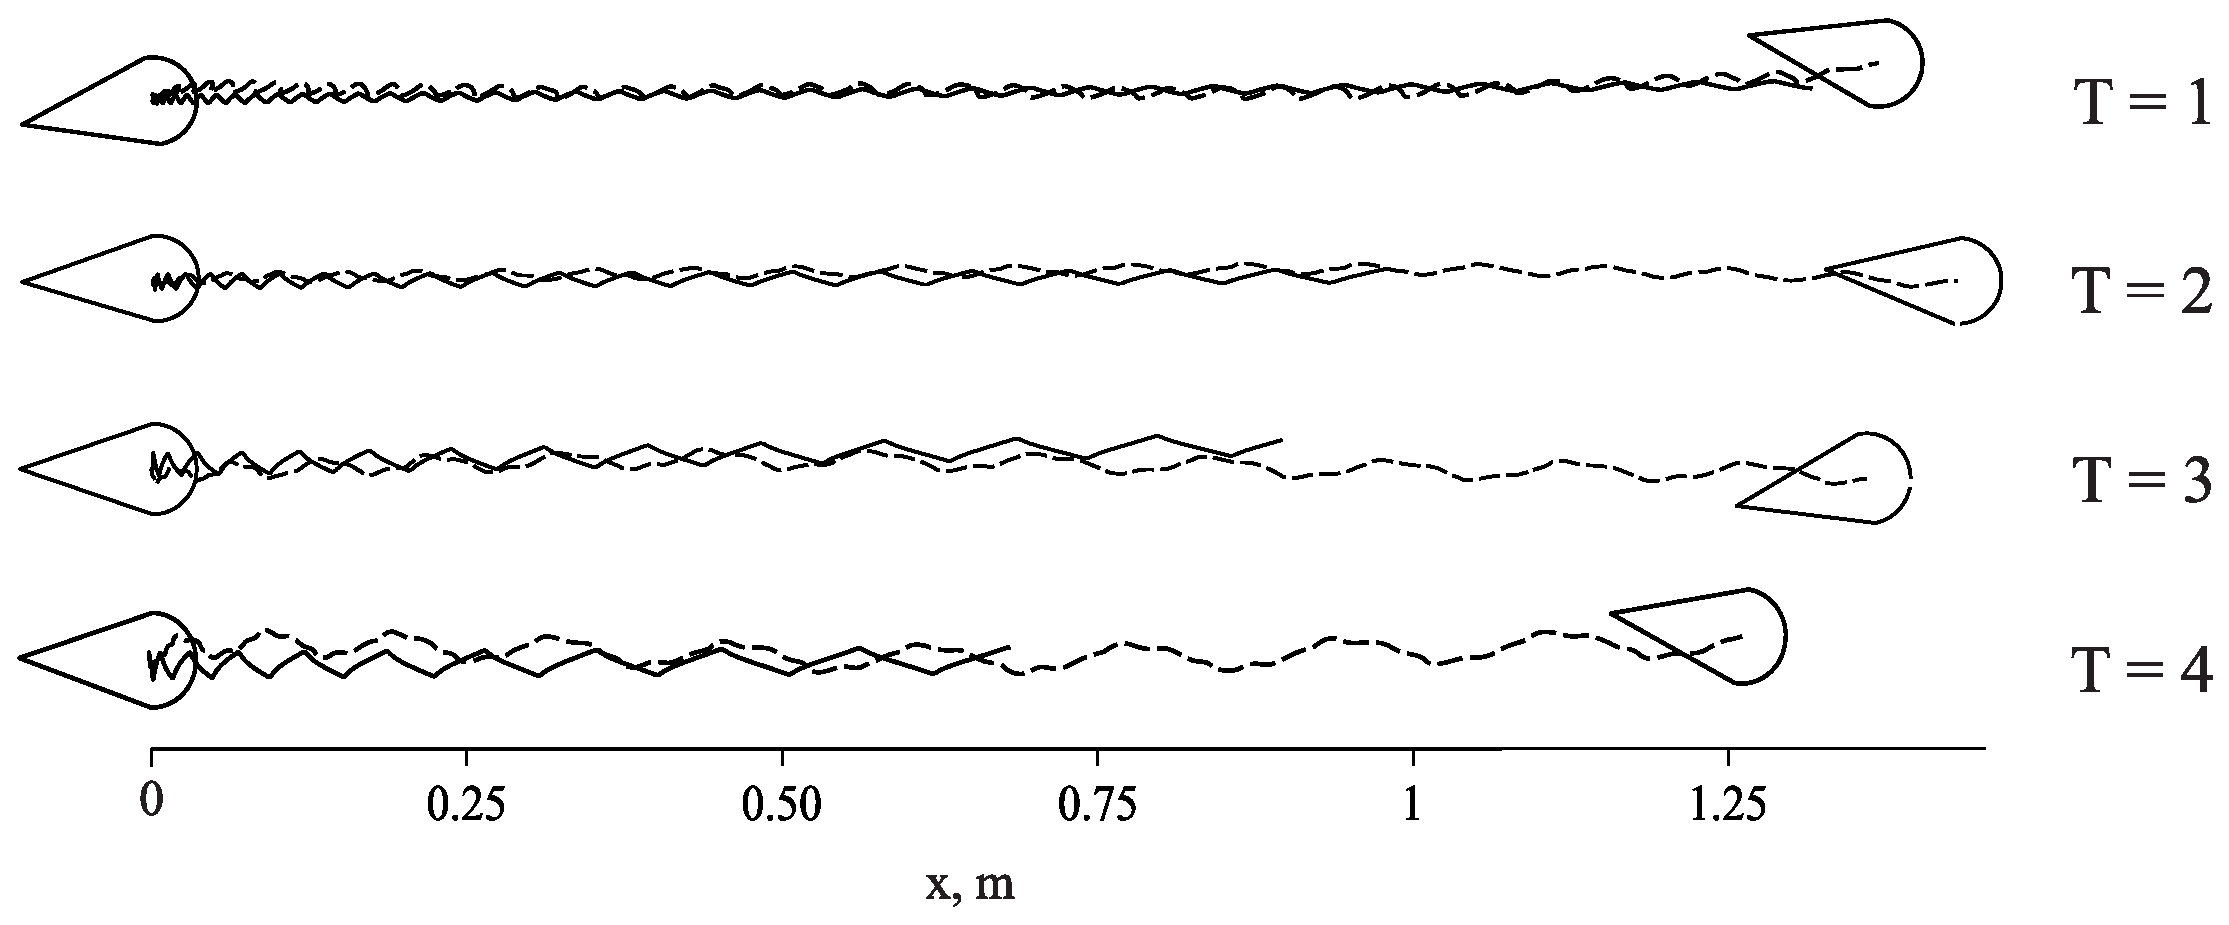
\includegraphics[width=0.9\linewidth]{AllTrajectories_new.eps} \\ }
	\end{minipage}
	\vfill
	\begin{minipage}[h]{0.3\linewidth}
		\center{а)}
	\end{minipage}
	\hfill
	\begin{minipage}[h]{0.7\linewidth}
		\center{б)}
	\end{minipage}
	\caption{а) График зависимости угловой скорости вращения ротора от времени в общем виде. $T$ --- период управляющего воздействия; $t_1, t_3$ --- интервалы времени с постоянными угловыми скоростями вращения ротора $\Omega_1$, $\Omega_2$ соответственно, $t_2$, $t_4$ --- интервалы равноускоренного вращения ротора. б) Траектории движения робота при  $ \Omega_1 = \Omega_{max} $, $ \Omega_2 = -\Omega_{max} $ и различных  управляющих воздействиях. Пунктирной линией обозначены траектории, полученные по результатам численного моделирования, сплошной~--- экспериментальные траектории.}
	\label{ControlAction}
\end{figure}

%\begin{figure}[!ht]
%	\centering
%	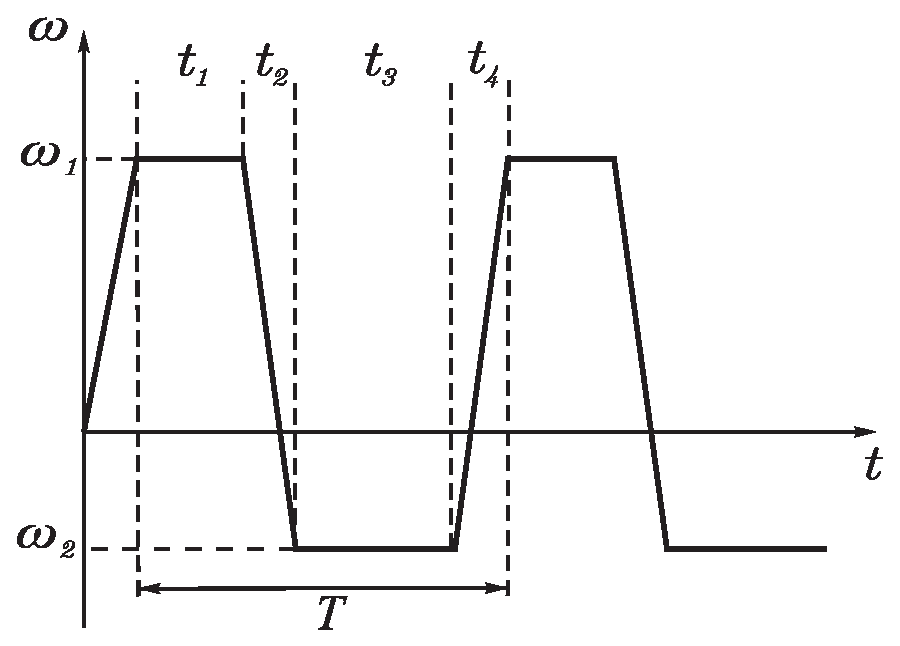
\includegraphics[width=0.35\linewidth]{ControlAction.eps}
%	\caption{График зависимости угловой скорости вращения ротора от времени в общем виде. $T$ --- период управляющего воздействия; $t_1, t_3$ --- задают интервалы времени с постоянными угловыми скоростями вращения ротора $\omega_1$, $\omega_2$ соответственно, $t_2$, $t_4$ --- интервалы равноускоренного вращения ротора.}
%	\label{ControlAction}
%\end{figure}

Далее на основании полученных уравнений движения и предложенного закона управляющего воздействия проведены исследования зависимости формы траектории от характера управляющего воздействия и от параметров прототипа робота. 
%Получены формы управляющих воздействий для движения вдоль прямой и вдоль окружности. 
%Показано, что для наиболее эффективного движения необходимо использовать ротор с максимально возможным моментом инерции при наименьшей массе, который расположен в центре масс системы.











В {\textbf{седьмой главе}} представлены результаты экспериментальных исследований движения в жидкости безвинтового надводного робота с острой кромкой.

Эксперименты проводились в бассейне 2 х 1.2 метра. При движении робота траектория отслеживалась с помощью системы захвата движения.% Vicon, которая состоит из 7 камер, расположенных по периметру бассейна.

\textbf{Движение вдоль прямой.} Проведем экспериментальные исследования со следующими параметрами, входящими в закон изменения угловой скорости вращения ротора: $t_1=t_3$, $ t_2 = t_4 \approx 0.1 $ секунды, $ \Omega_1 = \Omega_{max} $, $ \Omega_2 = -\Omega_{max} $, где $ \Omega_{max} $ -- максимальная угловая скорость вращения ротора для данной модели робота. Таким образом, в качестве изменяемого параметра в экспериментах движения вдоль прямой выступает период $T$. %, а $t_1=t_3 = 0.5(T - 2t_2)$. 
Проведены эксперименты при $ T = 1, 2, 3, 4 $ секунды. На рисунке~\ref{ControlAction}б представлены экспериментальные и расчетные траектории движения при различных управляющих воздействиях. 
%Так же схематично обозначена ориентация робота в начальный и конечный моменты времени. 
Время моделирования и экспериментов для всех тестов составило 40 секунд. %(вследствие ограниченного размера бассейна).

%Кадр с записи движения робота в бассейне представлен на рисунке~\ref{Frame1}. Как видно из рисунка, при данном управляющем воздействии робот движется вдоль прямой.
%
%\begin{figure}[!ht]
%	\centering
%	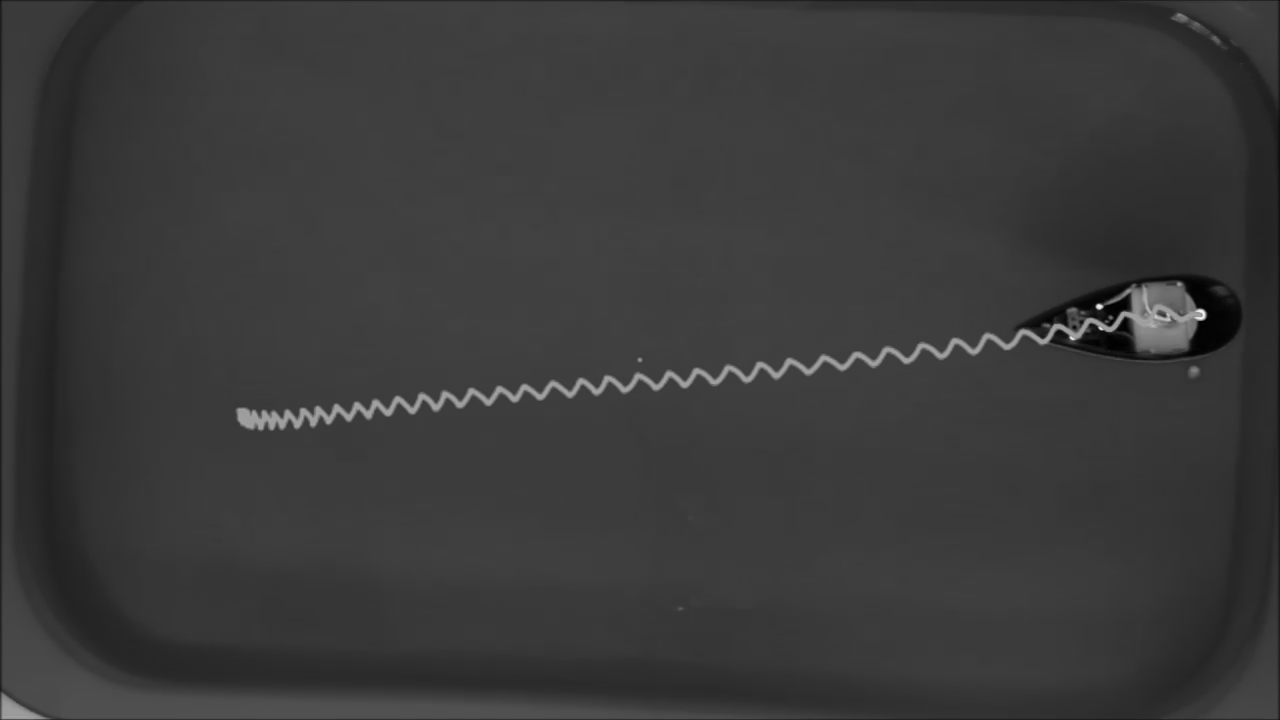
\includegraphics[width=0.7\linewidth]{Frame1.png}
%	\caption{Кадр с записи движения робота в бассейне}
%	\label{Frame1}
%\end{figure}



%\begin{figure}[!ht]
%	\centering
%	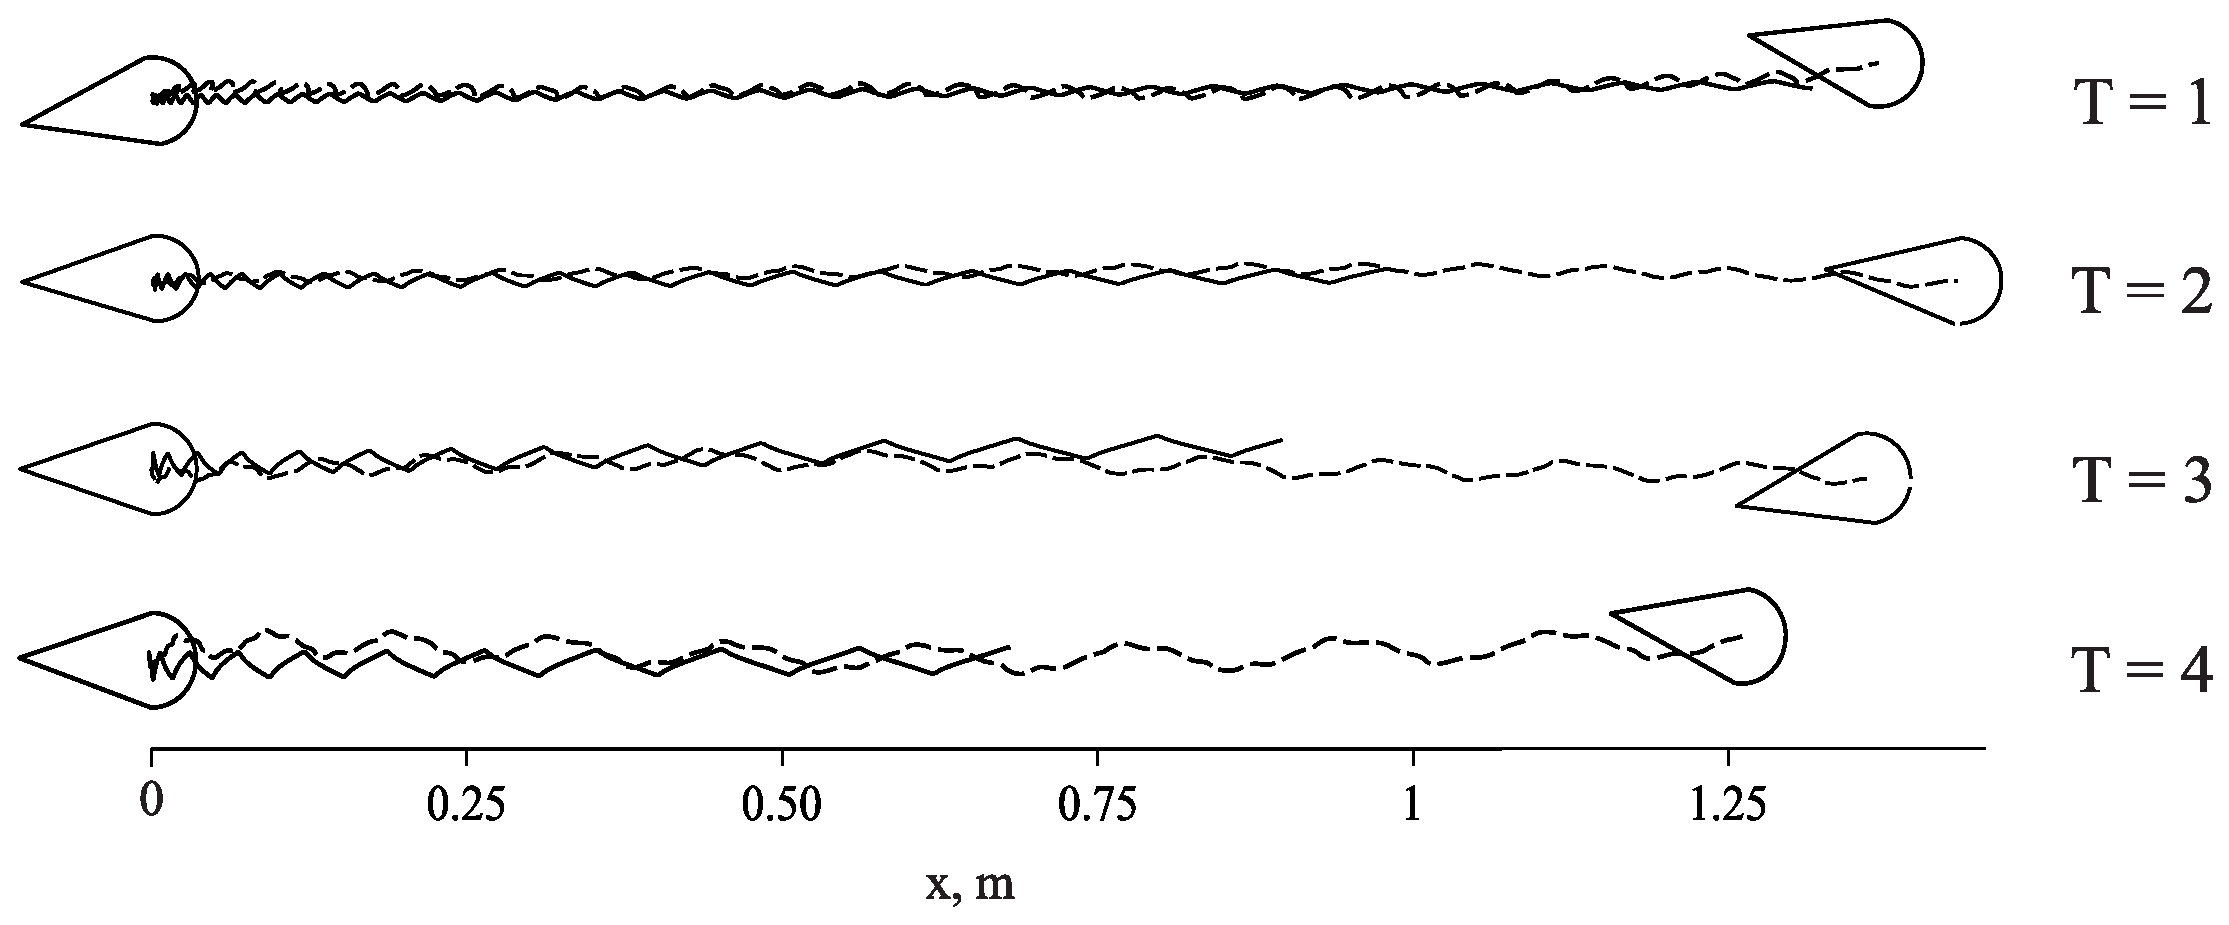
\includegraphics[width=0.65\linewidth]{AllTrajectories_new.eps}
%	\caption{Траектории движения робота при  $ \omega_1 = \omega_{max} $, $ \omega_2 = -\omega_{max} $ и различных  управляющих воздействиях. Пунктирной линией обозначены траектории, полученные по результатам численного моделирования, сплошной~--- экспериментальные траектории.}
%	\label{AllTrajectories}
%\end{figure}

Зависимость скорости движения робота от периода управляющего воздействия в данных исследованиях не очевидна, возможно, из-за ограниченных размеров бассейна. Наилучшее количественное согласование результатов моделирования с экспериментом получено при $T = 1$ c. Именно по этим экспериментальным данным проводилось вычисление коэффициентов модели. 
%Отклонение результатов моделирования от экспериментальных данных для других значений периода управляющего воздействия возможно минимизировать при уточнении значений коэффициентов модели для соответствующих условий эксперимента.

При смещении угловой скорости на величину $\Omega_0$ (см. рис.~\ref{DifferentAmp}а) и сохранении равенств интервалов $t_1=t_3$, $t_2=t_4$  робот также двигается вдоль прямой.  Соотношение угловых скоростей оставалось постоянным $ \Omega_1 - \Omega_2 = const$.  На рис.~\ref{DifferentAmp}б приведены соответствующие траектории движения робота, из которых видно, что робот двигался в среднем прямолинейно, но в различных направлениях. Причем изменение направления происходит в начале движения, а угол поворота зависит от сдвига управления $\Omega_0$. 

\begin{figure}[!ht]
	\begin{minipage}[h]{0.5\linewidth}
		\center{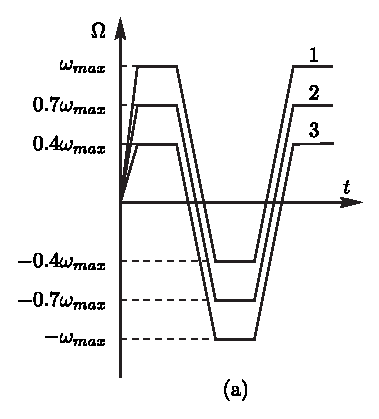
\includegraphics[height=0.65\linewidth]{ControlActionPlots3.eps} \\ }
	\end{minipage}
	\hfill
	\begin{minipage}[h]{0.5\linewidth}
		\center{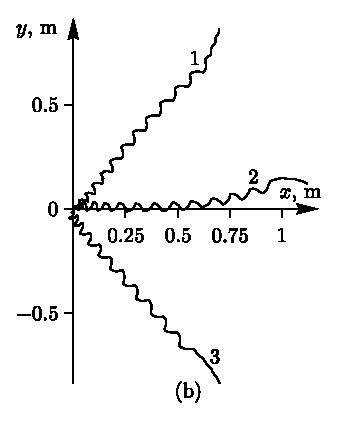
\includegraphics[height=0.65\linewidth]{Plots3.eps} \\ }
	\end{minipage}
	\vfill
	\begin{minipage}[h]{0.5\linewidth}
		\centering{а)} 
	\end{minipage}
	\hfill
	\begin{minipage}[h]{0.5\linewidth}
		\centering{б)}
	\end{minipage}

	\caption{Несимметричные управляющие воздействия при $\Omega_1 - \Omega_2 = const$, $t_2 = t_4 = 0.1$, $t_1 = t_3 = 0.9$, $T = 2$ (а) и соответствующие им траектории движения водного робота (б).}
	\label{DifferentAmp}
\end{figure}

%По результатам проведенных экспериментальных исследований можно сделать следующие выводы.
%\begin{itemize}
%	\item[-] Рассматриваемая теоретическая модель управляемого движения водного робота качественно правильно  описывает его движение вдоль прямой, которое реализуется симметричным управляющим воздействием.
%	
%	\item[-] Сдвиг управляющего воздействия $\Omega(t) \rightarrow \omega_0 + \Omega(t)$ не влияет на форму траектории, она остается прямой, но меняется направление движение.
%	
%	\item[-] Количественного согласования результатов моделирования и экспериментов можно достичь для конкретных тестов, проводя перерасчет коэффициентов под конкретные экспериментальные данные.
%\end{itemize}

\textbf{Движение вдоль окружности.} Движение робота по траектории по форме, близкой к окружности, оказывается возможным, если в управляющее воздействие внести ассиметрию на периоде. Ассиметрия достигается при $t_1 \neq t_3$ и $t_2 = t_4$. То есть длительности вращения ротора в направлениях по часовой стрелке и против часовой стрелки различны. Типовая траектория движения робота при $ t_3 = 10 t_1,\, \Omega_1 = \Omega_{max},\, \Omega_2 = -\Omega_{max},\, t_2 = t_4 = 0.1~\text{с},\, T = 3~\text{с} $
%\begin{gather}
%t_3 = 10 t_1,\quad \omega_1 = \omega_{max},\quad \omega_2 = -\omega_{max},\quad t_2 = t_4 = 0.1~\text{с},\quad T = 3~\text{с}
%\end{gather}
и результаты моделирования приведены на рис.~\ref{CircleTrajectory}а. На рис.~\ref{CircleTrajectory}б приведена графическая зависимость радиуса окружности, аппроксимирующей траекторию, от соотношения длительностей рассматриваемых интервалов $k_1 = t_3 / t_1$. 
%Для построения аппроксимаций расчетных и экспериментальных данных использовался метод наименьших квадратов.

\begin{figure}[!ht]
	\begin{minipage}[h]{0.25\linewidth}
		\center{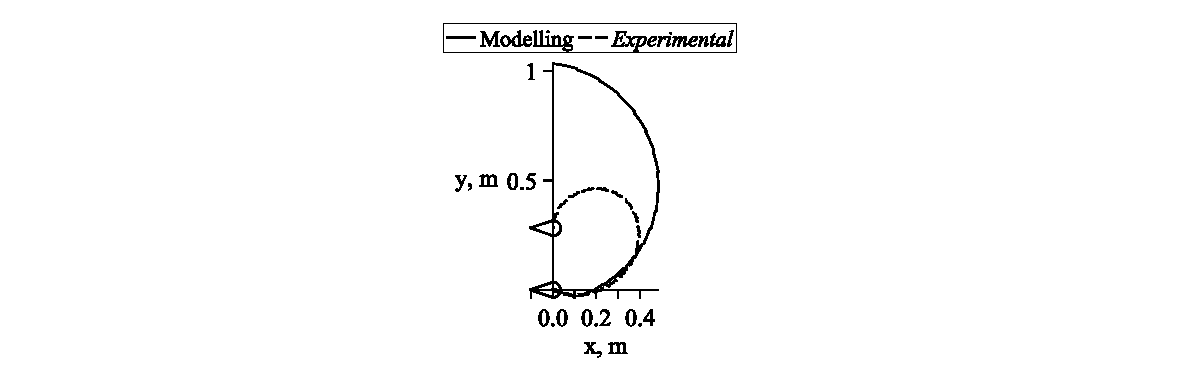
\includegraphics[width=0.65\linewidth]{xyCircleWmax.eps} \\ а}
	\end{minipage}
	\hfill
	\begin{minipage}[h]{0.6\linewidth}
		\center{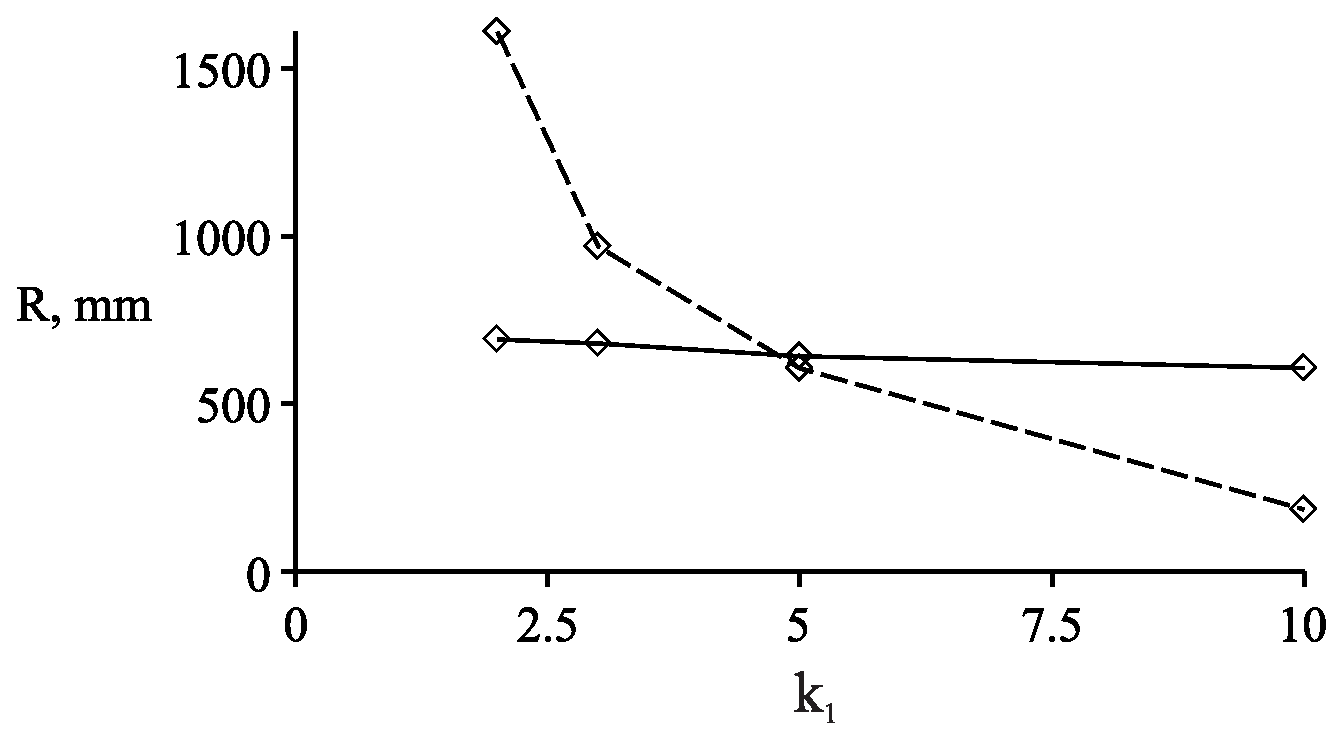
\includegraphics[width=0.75\linewidth]{kRDependence+Theor_T=3,W=max.eps} \\ б}
	\end{minipage}
	\caption{а) Траектория движения робота по окружности при эксперименте (штриховая линия) и моделировании (сплошная линия)  б) Зависимость радиуса траектории движения робота от $k_1 = \frac{t_3}{t_1}$ при эксперименте (штриховая линия) и моделировании (сплошная линия), построенная по экспериментам при $k_1 = 2,\ 3,\ 5,\ 10$ }
	\label{CircleTrajectory}
\end{figure}

%Форма расчетной и экспериментальной траектории качественно совпадают, но радиус окружности вдоль которой плывет робот при моделировании примерно в 2 -- 2.5 раза больше радиуса окружности, полученной в экспериментах.

Из рис.~\ref{CircleTrajectory}б видно, что теоретическая и экспериментальная зависимости качественно согласуются. 

Вторым способом достижения ассиметрии является форма управляющего воздействия при $t_1 = t_3$ и $t_2 \neq t_4$. На рис.~\ref{ControlActionOur}а представлены экспериментальная и расчетная траектории движения робота при данном управляющем воздействии для следующих значений: $ T=5,\, t_4 = 0.1,\, t_2 = 3,\, \Omega_1 = \Omega_{max},\, \Omega_2 = -\Omega_{max} $. На рис.~\ref{ControlActionOur}б приведены экспериментальная и расчетная зависимости радиуса траектории движения робота от коэффициента $k_2 = t_2 / t_4$. 
%Эксперименты проводились для $k_2 = 10,\ 20,\ 30,\ 40$.
%\begin{gather}
%T=5,\quad t_4 = 0.1,\quad t_2 = 3,\quad \omega_1 = \omega_{max},\quad \omega_2 = -\omega_{max}.
%\end{gather}

\begin{figure}[!ht]
	\begin{minipage}[h]{0.5\linewidth}
		\center{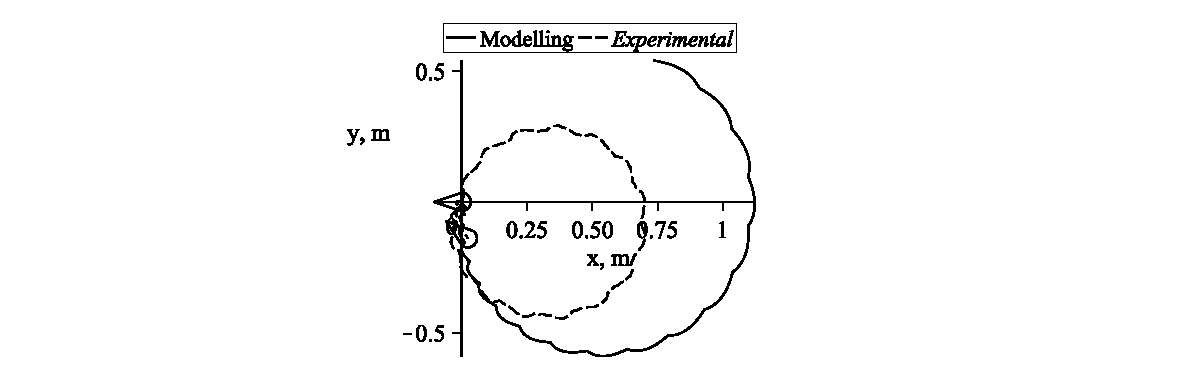
\includegraphics[width=0.55\linewidth]{xyCircleOur.eps} \\ а}
	\end{minipage}
	\hfill
	\begin{minipage}[h]{0.5\linewidth}
		\center{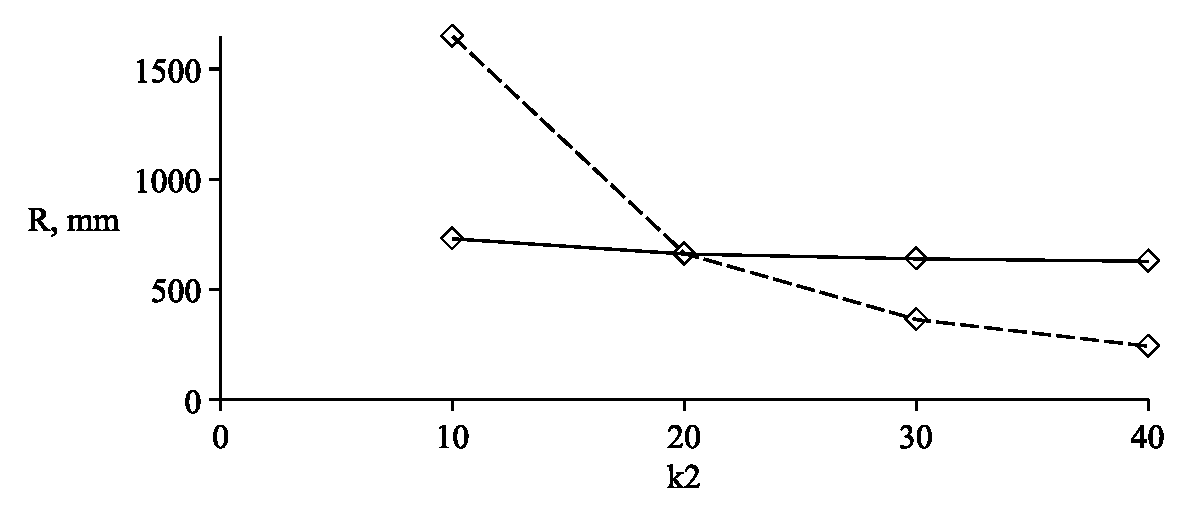
\includegraphics[width=0.98\linewidth]{nROur.eps} \\ б}
	\end{minipage}
	\caption{а) Траектория движения робота вдоль окружности при $T = 5$, $t_1 = t_3 = 0.95$, $t_2 = 3$, $t_4 = 0.1$, $\omega_1 = \omega_{max}$, $\omega_2 = -\omega_{max}$ в эксперименте (штриховая линия) и моделировании (сплошная линия), б) Зависимость радиуса траектории движения робота от $k_2 = \frac{t_2}{t_4}$ при эксперименте (штриховая линия) и моделировании (сплошная линия)}
	\label{ControlActionOur}
\end{figure}

Из рис.~\ref{ControlActionOur}б видно, что радиус траекторий, полученных при моделировании, незначительно уменьшается при увеличении $k_1$. Для траекторий, полученных в эксперименте, при увеличении $k_2$ в 4 раза радиус траектории уменьшается более чем в 6 раз.

%\begin{figure}[!ht]
%	\centering
%	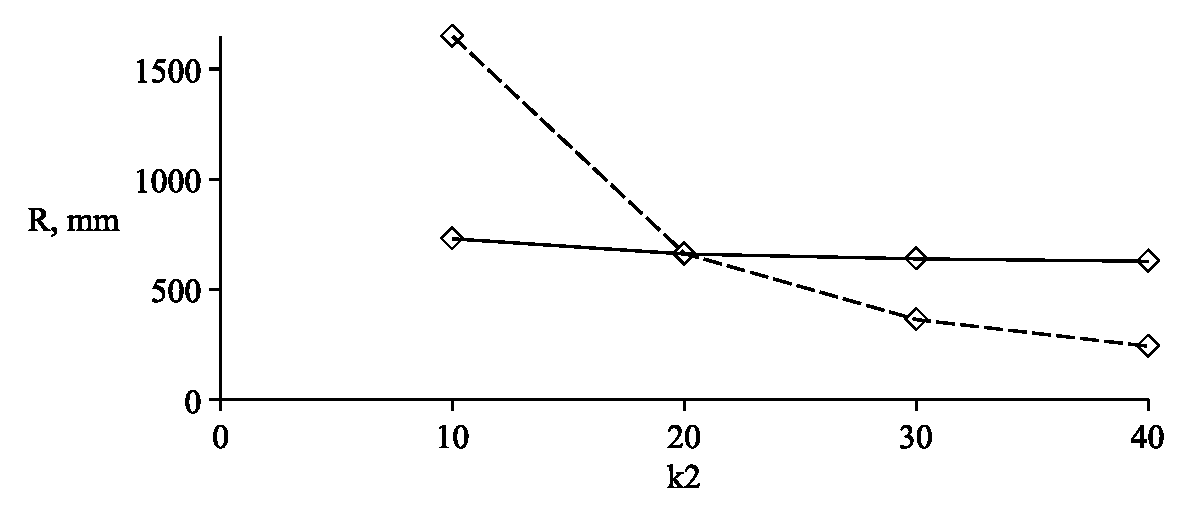
\includegraphics[width=0.8\linewidth]{nROur.eps}
%	\caption{Теоретическая (сплошная линия) и экспериментальная (штриховая линия) зависимости радиуса траектории движения робота от $k_2$ при $\omega_1 = \omega_{max} $; $ \omega_2 = -\omega_{max} $; $ t_1=t_3 $; $ t_4=0.1 $ секунды; $ T = 5 $ секунд}
%	\label{nROur}
%\end{figure}

При комбинировании рассматриваемых управлений, обеспечивающих движение вдоль прямой и окружности, можно реализовать движение вдоль сложных траекторий. На рисунке~\ref{Slalom} приведен пример управляющего воздействия и траектории, полученные в эксперименте и моделировании.

\begin{figure}[!ht]
	\begin{minipage}[h]{0.5\linewidth}
		\center{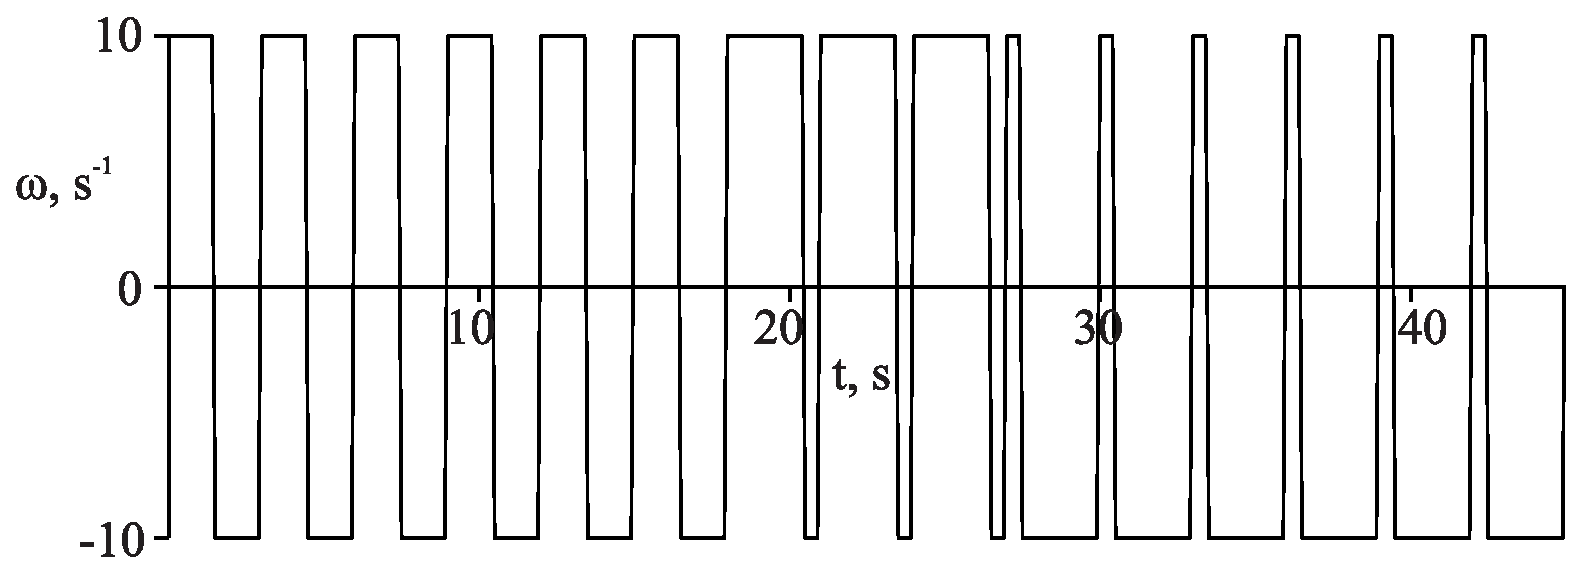
\includegraphics[width=0.9\linewidth]{ControlActionComplexTr.eps} \\ а}
	\end{minipage}
	\hfill
	\begin{minipage}[h]{0.5\linewidth}
		\center{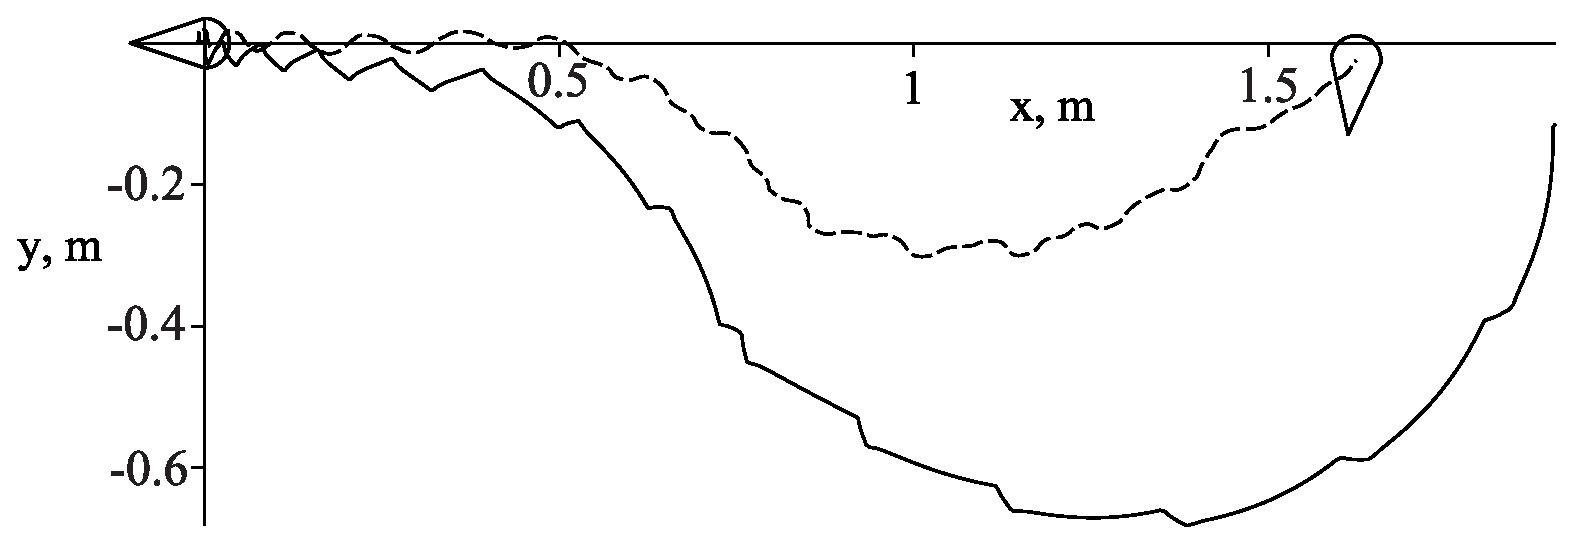
\includegraphics[width=0.9\linewidth]{ComplexTr.eps} \\ б}
	\end{minipage}
	\caption{Управления для реализации сложного движения (а) и соответствующая траектория движения (б)  при эксперименте (штриховая линия) и моделировании (сплошная линия)}
	\label{Slalom}
\end{figure}

Выделим основные результаты экспериментальных исследований:

\begin{itemize}
	\item Рассматриваемая теоретическая модель управляемого движения безвинтового робота качественно правильно  описывает его движение вдоль прямой и окружности. %Cимметричное управляющее воздействие -- движение вдоль прямой. Асимметричное управляющее воздействие -- движение вдоль окружности.
	
	\item Сдвиг управляющего воздействия $\omega(t) \rightarrow \omega_0 + \omega(t)$ не влияет на форму траектории. На размер и форму траектории движения влияет асимметрия управляющего воздействия на его периоде.
	
	\item Количественного согласования результатов моделирования и экспериментов можно достичь для конкретных тестов, проводя перерасчет коэффициентов под конкретные экспериментальные данные.
	
	\item Комбинируя описанные маневры, можно двигаться по сложной траектории.
	
	%\item [-] Количественного согласования результатов моделирования и экспериментов, как и в при движении вдоль прямой, можно достичь для конкретных тестов, проводя перерасчет коэффициентов под конкретные экспериментальные данные, полученные при движении вдоль окружности.
	
\end{itemize}



Полученные результаты подтверждают возможность теоретической модели качественно описать движение безвинтового робота, а также возможность формирования управления вдоль сложных криволинейных траектории, разбивая их на характерные участки, для которых можно сформировать базовые управления -- гейты. Одним из способов повышения точности совпадения количественных результатов численного моделирования и результатов экспериментов является уточнение коэффициентов модели для различных гейтов.

%Еще одним способом улучшить согласованность теории и эксперимента может быть более точный подбор формы для функции углового ускорения в моделировании. На рис.~\ref{OmegaT1EpsilonT1} для сравнения приведены аналитические (используемые при моделировании) и экспериментальные графики угловой скорости и углового ускорения ротора при $ T = 1 $ c. Видно, что графики для моделирования не полностью повторяют реальные зависимости, что приводит к неточностям в расчетах траектории.
%
%\begin{figure}[!ht]
%	\begin{minipage}[h]{0.5\linewidth}
%		\center{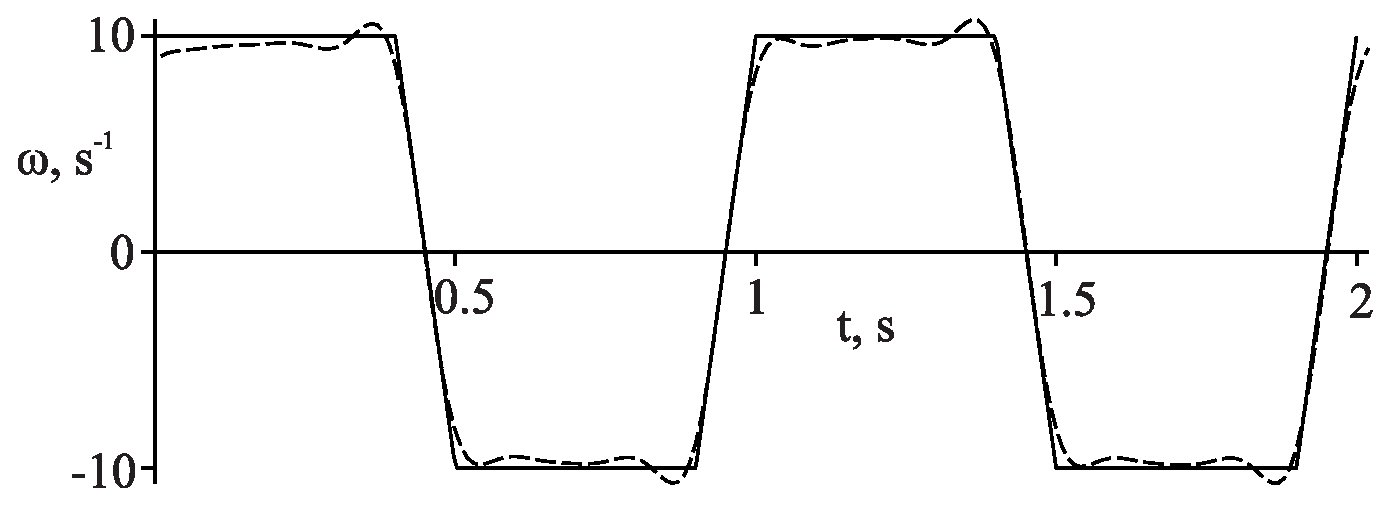
\includegraphics[width=0.9\linewidth]{OmegaT1Meandr.eps} \\ а}
%	\end{minipage}
%	\hfill
%	\begin{minipage}[h]{0.5\linewidth}
%		\center{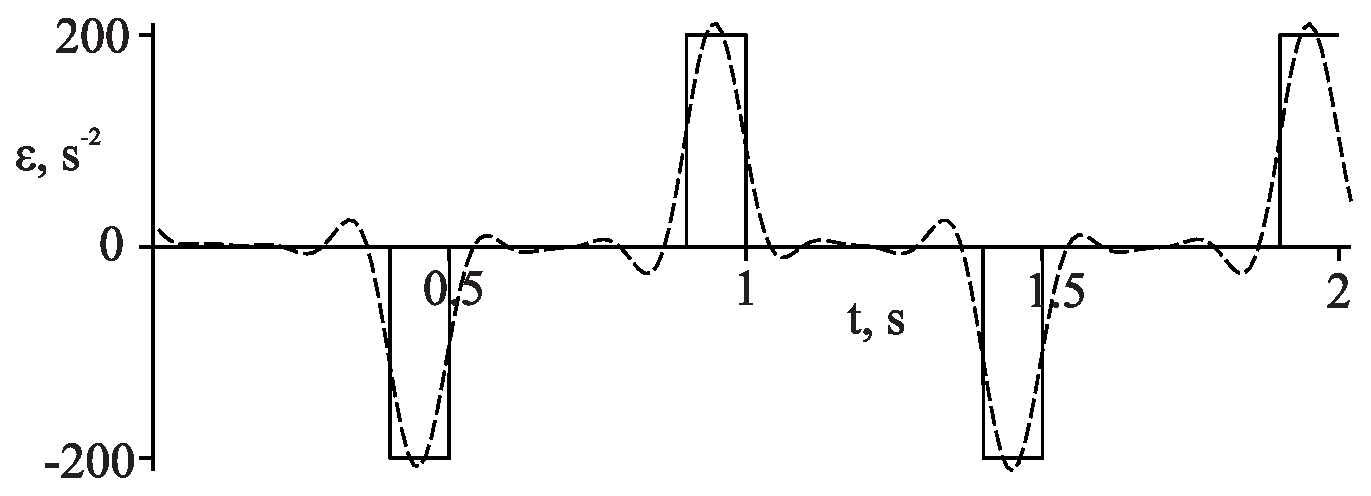
\includegraphics[width=0.9\linewidth]{EpsilonT1Meandr.eps} \\ б}
%	\end{minipage}
%	\caption{Зависимость угловой скорости ротора (а) и углового ускорения ротора (б) от времени при эксперименте (штриховая линия) и моделировании (сплошная линия)}
%	\label{OmegaT1EpsilonT1}
%\end{figure}

%Кроме того, повысить маневренность и управляемость движения водного робота можно с помощью модификации управляющего воздействия, обеспечив на интервалах $t_2,t_4 $ вращение ротора с разными ускорениями после смены направления вращения (см. рисунок \ref{gen_cont_ac}).    
%
%\begin{figure}[!ht]
%	\centering
%	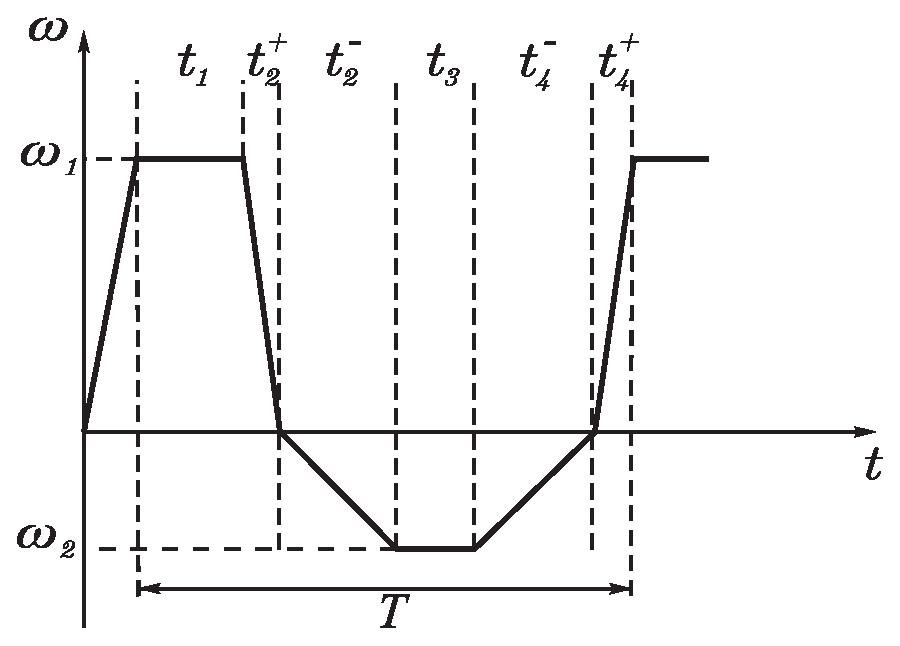
\includegraphics[width=0.5\linewidth]{ControlActionGeneral.eps}
%	\caption{Общий вид управляющего воздействия при различных ускорениях разгона и торможения}
%	\label{gen_cont_ac}
%\end{figure}





В {\textbf{заключении}} приведены основные результаты работы: %% Согласно ГОСТ Р 7.0.11-2011:
%% 5.3.3 В заключении диссертации излагают итоги выполненного исследования, рекомендации, перспективы дальнейшей разработки темы.
%% 9.2.3 В заключении автореферата диссертации излагают итоги данного исследования, рекомендации и перспективы дальнейшей разработки темы.
\begin{enumerate}
  \item Разработана математическая модель движения безвинтового подводного робота в форме эллипсоида в жидкости за счет внутреннего гиростатического момента в рамках теории идеальной жидкости. Исследования управляемости модели показали, что для полной управляемости форму робота необходимо сделать винтовой.
  
  \item Разработаны конструкция и экспериментальный образец безвинтового подводного робота в форме эллипсоида. Учтено требование в необходимости винтовой формы робота, к оболочке в виде эллипсоида вращения добавлены винтовые лопасти. Проработана конструкция внутренних компонентов с учетом ограничений в размерах. Разработана система управления роботом.
  
  \item Проведены экспериментальные исследования безвинтового подводного робота в форме эллипсоида, проанализированы результаты. Для более точного описания движения необходимо учитывать в модели вязкое сопротивление, генерацию вихревых структур. В рамках дальнейшего исследования рассматривается движение объекта в форме симметричного профиля NACA 0040 по поверхности жидкости.
  
  \item Разработана математическая модель движения безвинтового надводного робота с оболочкой, имеющей форму симметричного профиля NACA 0040 и острую кромку, в жидкости за счет внутреннего гиростатического момента с учетом вязкого сопротивления. На основе анализа математической модели разработан алгоритм управления роботом, определена форма управляющего воздействия для движения вдоль прямой и вдоль окружности.
  
  \item Разработаны конструкция и экспериментальный образец безвинтового надводного робота с острой кромкой. Разработана система управления роботом.
  
  \item Проведены экспериментальные исследования с безвинтовым надводным роботом с острой кромкой, проанализированы результаты. Показано, что разработанная математическая модель качественно описывает движение робота. Рассмотрены движения вдоль прямой и вдоль окружности при различных управляющих воздействиях.
  
  \item По разработанным конструкциям получен патент на полезную модель безвинтового подводного робота в форме эллипсоида, для разработанных программных продуктов получены свидетельства о регистрации программ ЭВМ.
\end{enumerate}




{
\setlist{leftmargin=6mm}
\vspace{2mm}

{\large  \textbf{Публикации автора по теме диссертации}}

\textbf{В изданиях из списка ВАК}
\begin{enumerate}	
	\item[1.] Ветчанин Е. В, Караваев Ю.Л., Калинкин А.А., Пивоварова Е.Н., \textbf{Клековкин А.В.} Модель безвинтового подводного робота //Вестник Удмуртского университета. Математика. Механика. Компьютерные науки. -- 2015. -- Т. 25. -- № 4. -- С. 544--553.
		
\end{enumerate}

\textbf{В изданиях, входящих в базу цитирования Web of Science}
\begin{enumerate}	
	\item[2.] Karavaev Y. L., Kilin A. A., \textbf{Klekovkin A. V.} Experimental investigations of the controlled motion of a screwless underwater robot // Regular and Chaotic Dynamics. -- 2016. -- Т. 21. -- №. 7-8. -- С. 918--926
	
	\item[3.] \textbf{А. В. Клековкин}. Моделирование движения безвинтового мобильного робота с неизменяемой формой оболочки управляемого с помощью вращения внутреннего ротора // Вестник Удмуртского университета. Математика. Механика. Компьютерные науки. -- 2020. -- Т. 30. -- № 4. С. 651--663. Принята к публикации.
	%\item[3.] Y. Karavaev, \textbf{A. Klekovkin}, I. Mamaev, V. Tenenev, E. Vetchanin. A Simple Physical Model for Control of an Propellerless Aquatic Robot // Journal of Mechanisms and Robotics. -- 2020. Направлена в журнал.
\end{enumerate}

\textbf{Патенты РФ}
	\begin{enumerate}		
		\item[4.] Патент на полезную модель. №172254 РФ. Безвинтовой подводный робот //  А.В. Борисов, И.С. Мамаев, А.А. Килин, А.А. Калинкин, Ю.Л. Караваев, \textbf{А.В. Клековкин}, Е.В. Ветчанин. Заявка: 2016144812, 15.11.2016, опубл. 3.07.2017
		
		\item[5.] № 2017613219. Программа для управления безвинтовым подводным роботом // А.В. Борисов, И.С. Мамаев, А.А. Килин, Ю.Л. Караваев, \textbf{А.В. Клековкин}. Заявка: 2016662663, 22.11.2016, опубл. 16.03.2017
		
		\item[6.] № 2019612284. Программа управления безвинтовым надводным роботом с внутренним ротором // А.В. Борисов, И.С. Мамаев, А.А. Килин, \textbf{А.В. Клековкин}, Ю.Л. Караваев. Заявка: 2019610925, 04.02.2019, опубл. 14.02.2019
	\end{enumerate}
}

%При использовании пакета \verb!biblatex! список публикаций автора по теме диссертации формируется в разделе <<\publications>>\ файла \verb!common/characteristic.tex!  при помощи команды \verb!\nocite!

%\ifdefmacro{\microtypesetup}{\microtypesetup{protrusion=false}}{} % не рекомендуется применять пакет микротипографики к автоматически генерируемому списку литературы
%\urlstyle{rm}                               % ссылки URL обычным шрифтом
%\ifnumequal{\value{bibliosel}}{0}{% Встроенная реализация с загрузкой файла через движок bibtex8
%  \renewcommand{\bibname}{\large \bibtitleauthor}
%  \nocite{*}
%  \insertbiblioauthor           % Подключаем Bib-базы
%  %\insertbiblioexternal   % !!! bibtex не умеет работать с несколькими библиографиями !!!
%}{% Реализация пакетом biblatex через движок biber
%  % Цитирования.
%  %  * Порядок перечисления определяет порядок в библиографии (только внутри подраздела, если `\insertbiblioauthorgrouped`).
%  %  * Если не соблюдать порядок "как для \printbibliography", нумерация в `\insertbiblioauthor` будет кривой.
%  %  * Если цитировать каждый источник отдельной командой --- найти некоторые ошибки будет проще.
%  %
%  %% authorvak
%  \nocite{Vetchanin_etc_Underwater_robot}%
%  %\nocite{vakbib2}%
%  %
%  %% authorwos
%  \nocite{Karavaev_Kilin_Klekovkin_RCD}%
%  \nocite{Karavaev_etc_2020} 
%  %
%  %% authorscopus
%%  \nocite{scbib1}%
%  %
%  %% authorconf
%  \nocite{Kalinkin_Klekovkin}%
%  \nocite{Klekovkin_Mamaev_GDIS_2016}%
%  \nocite{Klekovkin_MIKMUS_2018}%
%  \nocite{Klekovkin_Cheboksary_2019}%
%  \nocite{Klekovkin_Extreme_2019}%
%  \nocite{Klekovkin_Clawar_2020}%
%  %
%  %% authorother
%%  \nocite{patent1}
%%  \nocite{patent2}
%%  \nocite{patent3}
%%  \nocite{bib1}%
%%  \nocite{bib2}%
%
%  \ifnumgreater{\value{usefootcite}}{0}{
%    \begin{refcontext}[labelprefix={}]
%      \ifnum \value{bibgrouped}>0
%        \insertbiblioauthorgrouped    % Вывод всех работ автора, сгруппированных по источникам
%      \else
%        \insertbiblioauthor      % Вывод всех работ автора
%      \fi
%    \end{refcontext}
%  }{
%  \ifnum \value{citeexternal}>0
%    \begin{refcontext}[labelprefix=A]
%      \ifnum \value{bibgrouped}>0
%        \insertbiblioauthorgrouped    % Вывод всех работ автора, сгруппированных по источникам
%      \else
%        \insertbiblioauthor      % Вывод всех работ автора
%      \fi
%    \end{refcontext}
%  \else
%    \ifnum \value{bibgrouped}>0
%      \insertbiblioauthorgrouped    % Вывод всех работ автора, сгруппированных по источникам
%    \else
%      \insertbiblioauthor      % Вывод всех работ автора
%    \fi
%  \fi
%  %  \insertbiblioauthorimportant  % Вывод наиболее значимых работ автора (определяется в файле characteristic во второй section)
%  \begin{refcontext}[labelprefix={}]    \insertbiblioexternal            % Вывод списка литературы, на которую ссылались в тексте автореферата
%  \end{refcontext}
%
%
%  }
%}
%\ifdefmacro{\microtypesetup}{\microtypesetup{protrusion=true}}{}
%\urlstyle{tt}                               % возвращаем установки шрифта ссылок URL
%
%\hspace{-11mm}

	
